\documentclass[10pt,titlepage,a5paper]{book}

% \usepackage[babel,german=quotes]{csquotes}
 
 \usepackage[ngerman]{babel}
  \usepackage[utf8]{inputenc}
  \usepackage[T1]{fontenc}


 \usepackage{graphicx}
 \usepackage{geometry}
 \usepackage{pstricks}
 
% \usepackage[style=numeric-comp,backend=bibtex]{biblatex}
% \addbibresource{Bilbliothek.bib}
 
 \pagestyle{plain}
 
%\frenchspacing 

\parindent0em 
\parskip1.0ex plus 0.5ex minus 0.5ex
\sloppy

\geometry{left=2.5cm,right=2cm,bottom=3.5cm,top=2.0cm}

 \author{von\\[0.8ex]Felicitas Stotz}
 \title{\bf\Huge Die Horussöhne}
 
 \newcommand{\sterne}{\par{\centering ***\par}}

 \newenvironment{tg}{\begin{quote}\em}{\end{quote}}
  
 \newenvironment{dichter}{\begin{flushright}}{\end{flushright}}

\newcommand{\changefont}[3]{
\fontfamily{#1} \fontseries{#2} \fontshape{#3} \selectfont}



 \begin{document}
% .
% \newpage
% \newpage
 
 \changefont{ppl}{m}{n}
 
  %\maketitle
   
 \begin{titlepage} 

%\includegraphics[width=0.9\textwidth]{/home/felicitas/133_1.JPG}

\begin{pspicture}
(-4.9,8.5)
\rput(0cm,0cm){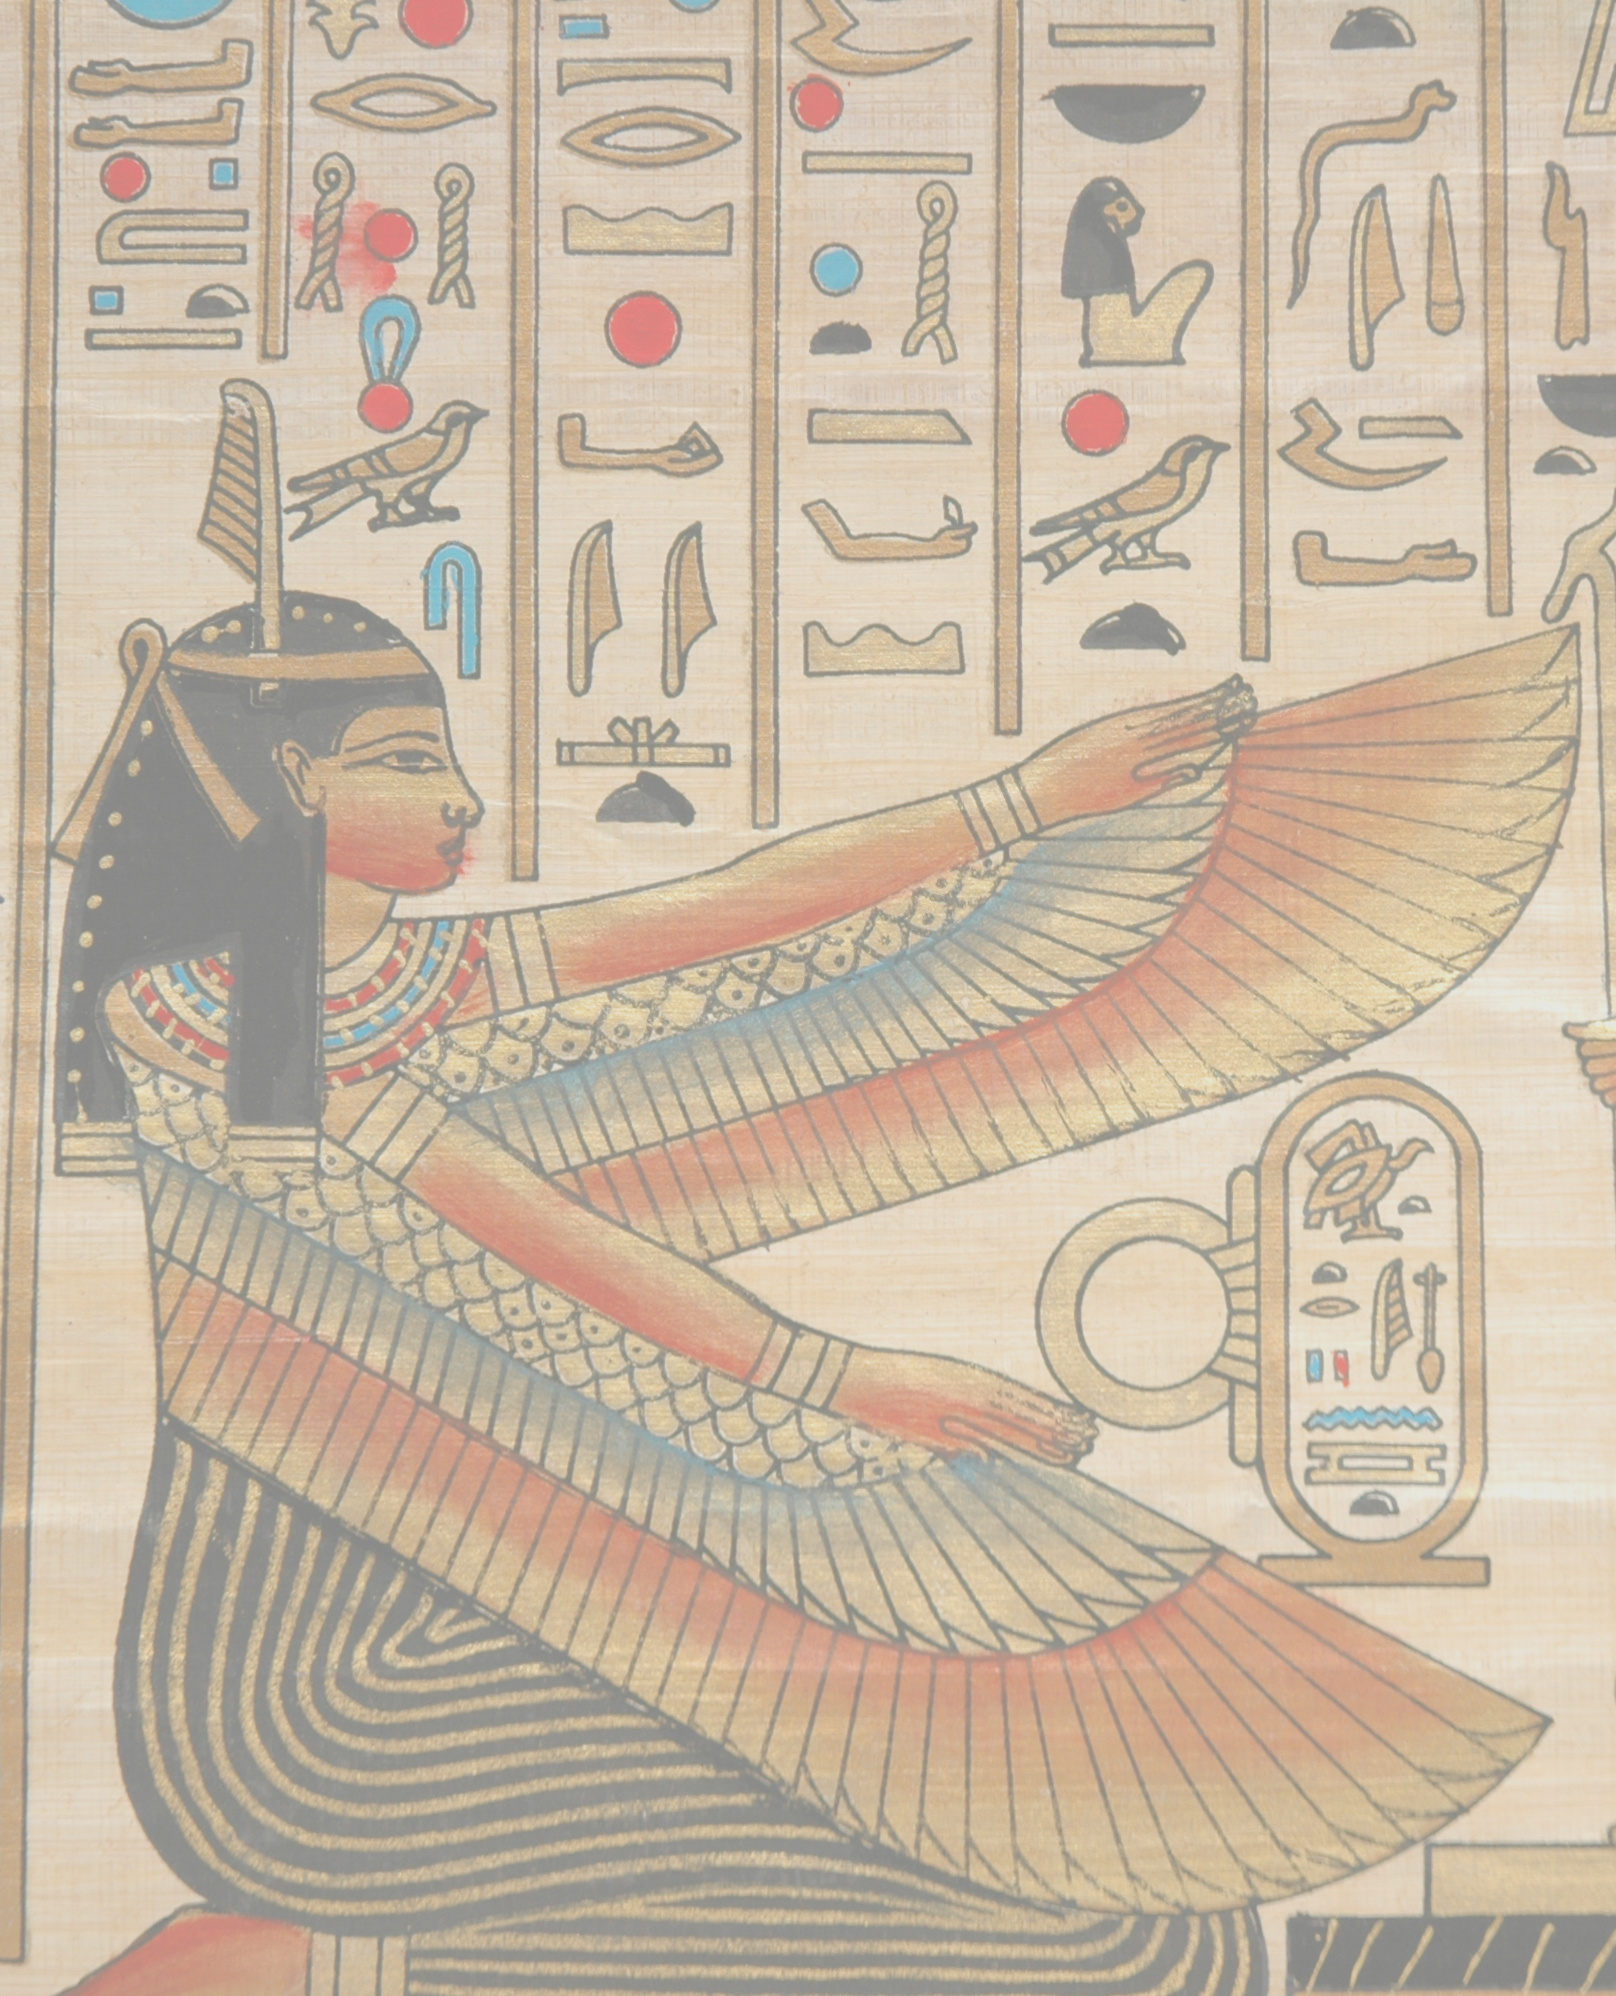
\includegraphics[width=\paperwidth,height=\paperheight]{Titel-Hell}}
\end{pspicture}
 
  \vspace*{-0.5\textheight}
   {\Huge\bf Die Horussöhne}\\[1.5ex]
   Felicitas Stotz\\[24.0ex]
   \today
 
 \end{titlepage}


\thispagestyle{empty}


\chapter*{}

\section*{Titelei}

\begin{tg}
\begin{verse}



Die Schrift des Verborgenen Raumes.\\
Die Standorte der Bau und der Götter,\\
die Schatten und Achu, und was getan wird.

Der Anfang ist das Horn des Westens,\\
das Tor des Westhorizontes;\\
das Ende ist die Urfinsternis,\\
das Tor des Westhorizontes.

Zu kennen die Unterweltlichen Bau,\\
zu kennen die Geheimen Bau,\\
zu kennen die Tore\\
und die Wege, auf denen der Grösste Gott wandelt.

Zu kennen, was getan wird,\\
zu kennen, was in den Stunden ist, und ihre Götter,\\
zu kennen den Lauf der Stunden, und ihre Götter.


Zu kennen ihre Verklärungen des RE,\\
zu kennen, was er ihnen zuruft,\\
zu kennen die Gedeihenden und die Ver\-nich\-te\-ten.{}\\

\end{verse}
\end{tg}



\chapter*{Prolog}
\addcontentsline{toc}{chapter}{Prolog}


Dies ist die Geschichte einer Reisegruppe. Da diese Reisegruppe aus Göttern besteht, handelt es sich um eine ungewöhnliche Reise und um ungewöhnliche Ereignisse und Abenteuer. Wenn Götter eine Reise machen und von dieser berichtet wird, dann verdienen sie ein Intro, einen Prolog, der ihnen angemessen ist. 

Alle Götter lieben es kreativ und innovativ zu sein, deshalb beginnen sie stets mit dem Anfang, der Schöpfung. Um die Darstellung unserer Schöpfung zeitgemäss zu präsentieren, wenden wir uns an einen besonderen Ort der modernen Götterverehrung, die im heiligen Wald, in the Holy Wood, Pardon, Hollywood\footnote{Holly= Stechpalme}. Die Götter mögen sie, denn die Menschen verwenden sie seit langer Zeit, um im Winter ihre Rauchfänge von bösen Geistern frei zu halten. Frag die Römer, Kelten, Germanen oder eben Angelsachsen drüben, hinterm grossen Teich oder den Dr. Botanicus, regelmässig zelebriert wird:

Das All!  Nicht das All, das wir kennen mit all den Lichtern und Blinkesternen, sondern das All vor Urzeiten, jung und neu. Wir sitzen in einem Raumschiff und beobachten, was passiert. Es ist dunkel, wie in Mutters Schoss. Die Panoramascheibe unseres Raumschiffes ist auf Nachsicht eingestellt. Alter Astronautentrick, um die Geburt von Planeten am Anfang allen Daseins und vor der Erschaffung des Lichtes zu beobachten.

Von der Kaffeemaschine tropft ein einzelner Tropfen herab, wir angespannt, zucken zusammen\dots und vor uns taucht majestätisch und langsam ein riesiger Planet auf. Er befindet sich an der Stelle, wo heute unsere Sonne ist und füllt den gesamten Platz zwischen Sonne und Saturn, so gross ist er. 

Langsam dreht er sich und wir bemerken unterschiedlich stark strahlende Felder. Wir sehen ein Zentrum in der Mitte, von eiem helleren umgeben und eine abschliessende Hülle darum. Eiförmige Gebilde  bewegen sich in dem Planeten. Wir schauen auf den Zeitmesser, der sich rasend durch die Zeit bewegt und 1000 Jahre in einer Millisekunde vorbeiziehen lässt. Die Zeit wird langsamer und wir schauen wieder raus. Es wird dunkler, es scheint als verlösche der riesige Planet. Nachdem er verschwunden ist, beschleunigt der Zeitmesser erneut. 

Und plötzlich erscheint vor unserem Panoramafenster ein neuer Planet an Stelle des alten. Dieser Planet ist kleiner und gasförmig. Wir können die Wärmesicht abschalten, wir sehen ihn wunderschön durch die Scheibe leuchten, wir tragen Sonnenbrillen, so hell leuchtet der Planet. Er strahlt glühend, leuchtend weiss, bis auf einige rauchig-dunkle Stellen, die aus Gas bestehen und dichter sind als der Rest. An einigen Stellen ballt sich Wärme, wie wir sie auf dem vorherigen Planeten gesehen haben.

Dieser Planet scheint zu atmen. Eine Zeitlang strömt das Licht weit in das All hinein. Angesogen von einer unsichtbaren Kraft und wird feiner und heller. Dann zieht es sich in das Zentrum zurück, dabei wird es dunkler, dichter, wie rauchige Luft. Kleine Gebilde kristallisieren sich darin, noch können wir sie nicht erkennen. Später werden sie die Sterne des Tierkreises bilden.

Wir haben die Zeit vergessen. Ein Blick auf unsere Zeitanzeige verrät uns, es sind Millionen Jahre vergangen. Wir schauen auf den Planeten und dieser ist wiederum in der Dunkelheit verschwunden.

Wir haben kurz Zeit uns einen Kaffee zu kochen und ein Schnittchen zu machen, da taucht an der Stelle ein neuer Planet auf. Er reicht von der Sonne bis zum Mars. Er ist fester als sein Vorgänger und schillert in allen Regenbogenfarben. Durch den Farbschleier sehen wir Nebel und durch den Nebel sehen wir zum ersten mal so etwas wie Leben. Eine grünliche Masse, wie gekochter Spinat, die lebendig ist und ab und zu ein "`Blubb"' von sich gibt\dots

Wir haben nicht viel Zeit dieses farbenprächtige Bild zu geniessen, denn die Masse des Planeten und die ganze Umgebung drumherum geraten in Aufruhr. Unsichtbare Kräfte reissen den Planeten auseinander. Während gleichzeitig das Universum von unsichtbaren Riesenhänden zusammengepresst wird. Zeitschlaufen öffnen sich und verschlucken Materie in dunklen Röhren, um sie an anderer Stelle auszuspucken. Unsichtbare, unglaublich starke Kräfte kämpfen gegeneinander. Trümmer fliegen herum, Feuerstürme toben, Luftlawinen wälzen sich durch den Raum.

Unser kleines Raumschiff ist zu dicht an dem Geschehen dran, es wird gepackt und geschüttelt. Wir purzeln durcheinander, es gibt eine riesige Kaffeesauerei und die lecker Schnittchen kleben an den Wänden. Draussen sehen wir Blitze, Gaswolken. Druckwellen schütteln uns. Ein riesiges Durcheinander findet statt. Der ursprüngliche Planet ist nicht mehr zu sehen.

Würden wir die alten Mysterien kennen, die ganze Ewigkeiten und durch viele Kulturen hindurch weitergegeben wurden, z.B. die Bhagavat Gita, würden wir wissen, in was wir hineingeraten sind: Den berühmten "`Streit im Himmel"'. Berühmt und berüchtigt, weil er die Geburt des Bösen beschreibt, das zu diesem Zeitpunkt nicht böse ist, sondern getrennt und allein.

- Gespenstische Stille-

Wir klopfen uns die Kleider ab, der Lehrling wird geschickt den Wischmop zu holen und die Kaffeepfützen zu entfernen und eine traurige Schinkenschnitte fällt von der Decke herunter.

Draussen hat es sich beruhigt, aber, was für ein Anblick!

An der Stelle des Planeten sehen wir eine Sonne, sie reicht nicht mehr bis zum Mars, dafür befindet sich auf der Marsumlaufbahn ein Mond. Er umkreist die Sonne und. Was auch immer die Turbulenzen verursacht hat, hat einen riesigen Ring an Trümmern hinterlassen, den Asteroidengürtel, den wir später zwischen Mars und Jupiter finden!

Die Sonne leuchtet hell und ist leicht, während sich auf dem Mond die Materie zu Luft und Wasser verdichtet. Auch hier schillern wieder die Regenbögen und der lebendige Spinat macht "`Blubb"'\dots

Ein letzter "Neustart" findet statt, Licht aus, Licht an und vor uns taucht die Erde auf. Sie ist viel grösser, denn es werden sich aus ihr Uranus und Saturn herauslösen, bevor sie sich endgültig verfestigt hat. Als nächster trennt sich der Jupiter und dann der Mars.

Wir können es nun wagen auf das Raumschiff zu verzichten, auch wenn wir bei der jetzigen Erdatmosphäre vermutlich einen Raumanzug nötig hätten, mit unserer heutigen Gestalt.
Ein letzter Blick auf den Zeitmesser, dort ist an Stelle der Zahlen eine Schrift erschienen: Genesis, Tag 1

Die Sonne verlässt die Erde und später, als letztes der Mond. Nachdem es sich die Planeten alle für diese Runde gemütlich gemacht haben, tritt das erste mal gross auf die Bühne in physischer Gestalt: Der Mensch.

Natürlich waren wir Menschen schon vorher da, wir waren auch dabei, als der Wärmeplanet sich im All begann zusammenzuballen, aber wir hatten kein Bewusstsein und nichts womit wir eines hätten haben können. Dieses Bewusstsein brauchte all die vielen Zeitrotationen auf unserem Zeitmesser, Millionen von Jahre und mehrere Äonen von Heimatplaneten, bevor es soweit war.

Und dann kam Atlantis. (Womit unsere Geschichte, der Leser möge den schmählichen, aber einkalkulierten Fauxpas verzeihen, einen Gènrewechsel von Science-Fiction zu Fantasy durchmacht, kommt nicht mehr vor, versprochen.)

Nebelverhangen war das Land Atlantis. Die Menschen besassen weder einen Körper, wie wir ihn kennen, noch hatten sie unser heutiges Bewusstsein. Die Menschen, sie träumten, sie fühlten sich, wenn sie wach waren, wie wir uns heute im Schlaf fühlten. Dabei waren die Atlantier hoch begabt, sie konnten etwas, was uns heute nicht mehr möglich ist. Sie waren hellsichtig und konnten die Kräfte, die im Pflanzen- und Mineralreich vorhanden sind, nutzten. 

Verrückt? Eigentlich nicht, wenn wir ein Auto anschauen, so nutzten wir dort Pflanzen- und Mineralkraft, indem wir das Auto aus Metall bauen und it Erdöl in Bewegung setzten.

Was die Atlantier jedoch tatsächlich unterschied und was uns heute am seltsamsten anmutet würde, ist nicht ihr merkwürdiger, zu Beginn dieser Zeit knochenlose Körper und ihre Hellsichtigkeit, die ihnen ein ähnlich komfortables, weitentwickeltes Leben wie uns heute, bescherte, nein, der grösste Unterschied war, sie kannten ihre Götter! Persönlich. Mit Vor- und Nachnamen und Adresse! (Was nicht fiel half, denn wie wir wissen, ging Atlantis kläglich unter.)

Einer, der nicht unterging, so sagt es die Legende, weil er weise war und sich deshalb dem wohlwollen der atlantischen Götter erfreute, war Thot. Thot, der später selbst Gott im Ägypterland wurde und auch bei den Griechen kein unbekannter war. im Gegenteil, sie nannten ihn, wiederum nach ihrem Gott Hermes: Hermes Trismegistos. Wer jetzt im hinterletzten Winkelchen seines Gehirns ein leises Klingeln hört, das sich wie "`hermetisch"' anhört, dem wird dämmern, wie weitreichend Thots Einfluss war und ist. Dabei ist er nicht der mächtigste der ägyptischen Götter\dots

Er ist allerdings der Gott, weil mit dem Menschlichen wohl vertraut, der sich am besten als Reiseleiter eignet. Für eine Reisegruppe von Göttern, die teilweise nicht über menschliche Körper verfügen, oder nie aus dem Jenseits, der ägyptischen Duat herausgekommen sind.

 Der Jenseitsbereich ist um die Erde herum, ein riesiger Raum für alle Götter, die für die Erde zuständig sind. Allerdings haben die Götter des einen Zeitalters und/oder des einen oder anderen Landes ihre ganz spezifischen Aufgaben und nicht alle, wollen sich um alles kümmern, andere haben sich auf den "`Altenteil"' zurückgezogen und geben den jüngeren Göttern Tipps, wie man tüchtige Blitze schleudern kann, ohne dabei die ganze Gemeinde auszulöschen.
 
 Wenn sich die Menschen jedoch anmassen, sich einem Gott zu widersetzten, oder einen unbestechlichen Wächtergott auf grausame Weise hintergehen und seinen schutzbefohlenen schaden, dann können auch alte Götter sich für eine Reise entschliessen. Und nicht alle Götter scheuen sich, ihre Kollegen um Hilfe zu bitten. Und so kommt es, dass der grosse Hermes Trismegistos, der "`dreimal grosse Hermes"', genannt Thot, gleich in dreifacher Mission nach Basel kommt.

Im berühmten Oktagon, dem achteckigen Zimmer des weissen Hauses des ehrwürdigen Jakob Sarasin, trifft sich der alte ägyptische Gott mit seinen nordischen Freunden Berta, auch bekannt als eine gewisse, Frau Holle und Hans, der als "`Wildr Maa"' der Gastgeber in Basel ist.
\sterne
 
"`Interessant, äusserst interessant!"' Thot legte die schlanken Fingerspitzen aneinander. "`Und was schliesst du daraus, verehrte Berta?"' "`Lieber Thot, wenn ich es selber wüsste, hätte ich Euch wohl kaum hierher bemüht!"' "`Och, im Moment werde ich gerne bemüht, es ist langweilig geworden."' 
"`Meine Herren, ich bin sicher, dem können wir abhelfen. Da ist etwas ganz finsteres im Gange, das hab ich in den Knochen. Hans? Hans, was sagst Du dazu?"' "`Wckl? Was?"' "`Herrjeh, dann hat er einmal im Jahr seinen grossen Auftritt und danach ist er Wochenlang nicht zu brauchen. Dir tut etwas mehr Bewegung gut, alter Mann!"' "`Alter Mann?! Also nai, Berta, eso nit!"' "`Fein, dann ist es beschlossen?"' Thot schmunzelte, sie waren sich überall ähnlich, die alten Herrschaften \dots

"`Wo? Ich persönlich würde Europa vorziehen, da ich selbst etwas erledigen will, was in Ägypten nicht möglich ist!"' "`Hans? Was meinst Du?"' "`Basel! Lasst es uns in Basel machen. Die Basler sind fromm genug geblieben und gleichzeitig  ignorant und mit sich beschäftigt, da fallen ein paar Götter mehr oder weniger nicht auf. Hermes hat da alte Kontakte. Ich hab Kontakte dort  und dir, liebste Berta, liegt das ganze Dreiländereck zu Füssen."' "`Gut, klingt vernünftig, auch, wenn es von dir kommt!"' "`Berta! Eso, würkli nit!"'    

"`Das Wann dürfte allen klar sein?"' "`Berta!"' "`Natürlich, liebe Berta!"'
"`Ja dann, see you later mit alligator\dots, haha!"' "`Bis Mitwinter!"' "`Es sind Krokodile! Keine Alligatoren, sondern Krokodile. Bis Heilig Abend."'



\part*{Erste Stunde:\\"`Welche die Stirnen der Feinde des Re zerschmettert"'}
\addcontentsline{toc}{part}{Erste Stunde}


\chapter*{24.Dezember; Adam und Evatag}
\addcontentsline{toc}{chapter}{24.Dezember; Adam und Evatag}

\section*{1}
"`Hermes, alter Junge, in diesem Moment wird Berta alles für den Transport vorbereiten. Sind wir bereit?"' "`Wir sind bereit, Hans. Unsere grosszügigen Gastgeber haben uns freundlicherweise ihre beiden Häuser zur Verfügung gestellt, die auf das beste geeignet sind."' "`Is' denn Alessandro fertig mit seinem Schutznetz? Hat er die Zeitüberschneidung richtig berechnet?"' "`Ja, ich habe es überprüft. Und unser Alessandro ist ein wahrer Spezialist, wenn es darum geht einen Ort in zwei Zeitzonen einzuteilen. Schliesslich ist diese Fähigkeit sehr nützlich, wenn man, wie er, gerne dem schönen Geschlecht huldigt."' "`Ei, das hesch schön gesagt, dem 'schönen Geschlecht' huldigen\dots so isses, Hermes, der Herr Graf ist kein Kind von Traurigkeit, das isch wahr!"' 

"`Die Häuser werden in der Gegenwart am Tag benutzt, auch das ist ein Vorteil. Vielleicht wird der eine oder andere Mensch Kopfschmerzen haben und wirre Träume, aber mit dem können wir leben."' "`Gut, dann werde ich Berta sagen, dass wir unseren Transport starten können und ihr helfen, die Route frei zu halten und den kleinen Krabbelviechern Beine machen. Hermes, viel Glück bei eurer Reise, deine Herrschaften sind ja nicht mehr die jüngsten."' "`Du solltest sie sehen, die gute Hathor, ist schon seit Wochen am Packen. Sie freuen sich alle auf das Abenteuer."' "`See you\dots"' "`Es sind Krokodile, Hans. Bis bald."'

\sterne

Amélie öffnete die Augen, was für ein Traum\dots

Aber, he, das war nicht ihr Zimmer! Wo in aller Welt war sie? Sie zog die weisse Bettdecke, die mit den Daunen von einer Million Gänsen gefüllt war, herauf zur Nasenspitze und rutsche tiefer in das weisse, flaumige Kissen. Sie lauschte, während die Augen das Zimmer durchstreiften. 
Die Wände waren weiss. Eine Kommode aus Nussbaum stand an der einen Wand, das Bett an der anderen. Am Kopfende des Bettes fiel durch ein grosses Sprossenfenster trübes, graues Winterlicht, in den langen schmalen Raum. Durch die Tür, gegenüber dem Fenster, hörte sie eilige Schritte hin und her gehen. Das Zimmer schien sich in einem grösseren Gebäude zu befinden. Stimmen waren zu hören. 

Das Zimmer roch nach Wachs mit dem der dunkle, alte Holzboden gepflegt worden war. Es roch nicht nur alt, sondern unpersönlich, wie ein Büro- oder Amtsgebäude. Die Geräusche und Stimmen schienen einer aufgeregten Grossfamilie zu gehören.

Amélie streckte sich. Und starrte an die Decke. An der Decke war ein schwarzer Punkt. Ein schwarzer Punkt, der sich bewegte! Eine Spinne? Amélie steckte den Kopf unter die Decke. Vorsichtig spähte sie hervor, der Punkt war weg! Mit einem kleinen Schrei, sprang Amélie aus dem Bett. Schüttelte sich wild und hopste durch Zimmer. Dann schaute sie hektisch, ob die Spinne an ihr klebte. Wo war die verdammte Spinne? Über der Kommode, ein schwarzer Fleck, Amélie sah genauer hin, es war keine Spinne, es war eine Ameise. Überrascht betrachtete Amélie sie genauer. Eine Ameise? Im Winter? Amélie beugt sich vor, ihre langen, glatten schwarzen Haare rutschen über die Schultern nach vorne. Diese Ameise sah erschöpft aus!

Amélie setzte sich auf das Bett, sie hatte ein weisses Unterhemd mit breiten Spitzenträgern und eine weisse Unterhose an. Kalt war es, sie schlang die Arme um sich und zog die Beine an. Sie versuchte sich an den Traum zu erinnern, darin kamen Ameisen vor. Sie hatte geträumt, eine riesige Zahl Ameisen würde sie durch einen unterirdischen Gang schleppen. Sie wurden von einem grossen, kräftigen Mann mit einem dunkelbraunen, struppigen Vollbart und wildem Haar angetrieben, der mit grünem und braunem Laub bedeckt war. Amélie war betäubt, sie konnte sich während des Transportes nicht bewegen, dämmerte auf dem Marsch dahin, der, wie ihr schien, Tage dauerte. Einzig geweckt wurde sie, wenn ihr Kopf oder ein anderer Körperteil unsanft gegen eine Baumwurzel schlug, die  in den erdigen Gang hineinragten. Sie erinnerte sich an grässlichen Lärm quietschender Räder auf Schienen. Tunnel, dunkel, betoniert und mit Leitungen vollgestopft. Ein blendendes Licht, S-Bahnen, die direkt auf sie zu gebraust kamen und mitten durch sie, die Ameisen und den fluchenden, wilden Mann hindurchfuhren, ohne abzubremsen. Und in dem Tunnelgewirr verschwanden, während die Ameisen sie mit dem Kopf solange gegen die Wand stiessen, bis diese nachgab und sie sich wieder in dem Erdgang befanden.

Es klopfte an der Zimmertür.
"`Hallo? Amélie! Bist Du wach?"' Amélie rutschte unter die Decke. Panik machte sich breit, das war eindeutig die Stimme von einem Kerl, einem jungen Kerl. Sie hörte angespannte Stille, dann schnüffelte es an der Tür. "`Ja! Nein! Stopp!"' rief Amèlie, aber da stand der junge Mann in der Tür und an ihm vorbei drängelte sich ein graziler, schlanker Hund mit dickem, goldbraunem Fell. Er trug einen schwarz-grauen Sattel aus längerem Haar auf dem Rücken und die Ohren waren spitz und gross. Der Hund war es, der aufgeregt schnüffelte. Er blieb in einiger Entfernung stehen und starrte Amèlie unhündisch an.

"`Ich hab keine Kleider,"' Amélie spürte, wie ihr die Röte ins Gesicht stieg und verschwand unter der Decke. "`Ah, oh! Ich glaube Isis hat dir etwas zum anziehen in die Kommode gelegt."' Sagte der junge Mann zu der Bettdecke. "`Ich bin übrigens Amset und das ist mein Bruder Duamutef, er ist ein Schakal."' 

Isis? Sein Bruder? Ein Schakal? Hilfe, bin ich von Verrückten entführt worden? Vorsichtig schob Amèlie ihre Nase hervor und rief empört: "`Du bist ja immer noch da! Verschwinde! ich will mich anziehen!"' Amélie nahm das Kissen und warf es, es prallte an der hastig geschlossenen Tür ab und plumpste zu Boden.

-Haha, sie hat nach fünf Minuten schon den ersten Gegenstand nach dir geworfen, Amsi! -Ach, halt dein Maul, Tef! -Hast du gewusst, dass sie dich für verrückt hält? -Maul halten, Tef! -Haha! Der Schakal und der junge Mann stiegen die grosszügige Treppe hinunter. Sie waren Götter und Brüder, der eine war ein junger Mann und der andere hatte die Gestalt eines Schakals. Wie sie miteinander sprachen? Mit Gedanken! Sie waren sogar vier Brüder, die berühmten Horussöhne, unbestechliche Wächter im Totenreich. Der dritte Bruder Kebechsenuef hatte Falkengestalt und der vierte, Hapi, die eines Pavian.

-Geh raus in den Garten deine Geschäfte machen, Tef! Und Grüss Hapi und Kebi von mir. -Heb' mir was vom Frühstück auf, ja? Der Schakal verschwand durch die Tür, die Amset ihm öffnete, in den Garten.

Amélie tappte auf Zehenspitzen zur Kommode. Aus dem Augenwinkel bemerkte sie eine Bewegung am Fenster. Es war nichts zu sehen. Ausser dem grauen Himmel.

 "`Gib sie her!"' "`Hol sie dir doch! Komm doch! Kooomm!"' "`Isfet, gib sie her, ich bring dich um!"'"`Vergiss es, Maat, das darfst du garnicht!"' Die Tür flog auf und zwei Mädchen fielen ins Zimmer. Sie wälzten sich am Boden. Die eine von ihnen hielt eine weisse Straussenfeder von sich gestreckt, nach der die andere hektisch griff. Sie bekam sie nicht zu fassen, weil ihre Gegnerin energisch zappelte. Amélie schnappte sich behutsam die Feder und zog sich ans Fenster zurück. "`Gib mir die Feder!"'

Die schlanke Gestalt, etwas kleiner als Amélie, streckte gebieterisch die Hand aus. Sie trug ein gerade geschnittenes, schwarzes Kleid mit weissem Spitzenkragen. Sie hatte weisse Söckchen ebenfalls mit Spitze an, im Winter! Und schwarze Spangenschuhe aus Lack. Die schwarzen Haaren trug sie zum Pagenkopf geschnitten, mit einer weissen Schleife gebunden. Die Haare waren zerzaust und die Schleife hing schief, ihre Wangen waren gerötet. Aber als sie ihr in das Gesicht sah, bekam Amélie eine Gänsehaut.

 Ihre Augen waren gelb. Goldgelb. Und sie strahlten eine machtvolle Würde und Weisheit aus. Amélie schluckte und gab dem Mädchen die Feder, stumm und erschrocken. "`Danke!"' sagte die zarte Person und ging erhobenen Hauptes aus dem Zimmer. 
 
 "`Isfet!"' sagte die andere und streckte Amélie die Hand entgegen. Diese hätte ein Zwilling sein können, allerdings einer, der aus dem Nest der Ordnung gefallen schien. Isfet hatte kurze, verwuschelte, schwarze Haare. Sie steckte in einem riesigen, bunten Sweatshirt mit Kapuze und einem Pinguin drauf, ihre Beine in pinken Leggings mit blauen Tupfen und die Füsse in dicken Stiefeln.
 
"`Amélie,"' sagte Amélie. "`Ich weiss!"' Isfet liess sich auf das Bett fallen. "`Alle scheinen das zu wissen"', maulte Amélie "`und ich weiss nicht mal, wo ich bin. Verdammt, wo bin ich und wer seit ihr? Ein Haufen Verrückte?"' Isfet grinste: "`Du bist schon in Ordnung, weisst du das? Zieh dich an und komm runter, dann lernst du den restlichen Haufen kennen."'

Amélie zog die Kommodenschublade auf, da! Da war wieder eine Bewegung am Fenster, sie zuckte zusammen. Isfet jedoch sprang ans Fenster, riss es auf und schrie: "`Kebi, lass' das, sie ist ein Mädchen und ein Gast, n' bisschen Anstand, jaah!"' Sie schloss das Fenster wieder und drehte sich zu der bleichen Amélie. "`Diese Brüder. Wenn sie nicht arbeiten, sind sie immer zu Spässen aufgelegt, die Jungs!"' Isfet ging aus dem Raum und Amélie trat ans Fenster. Auf dem gegenüberliegenden Dach sass ein Raubvogel, ein Falke. Komisch, dachte Amélie, mitten in der Stadt\dots

 Brüder? Hatte jemand von der gegenüberliegenden Seite aus dem Fenster geschaut? Amélie betrachtete das Haus. Es erstreckte sich auf drei Seiten. Zwei Stockwerke war es hoch und im Dach waren viele kleine Gauben mit weiteren, kleinen Fenstern. Blau, weiss war das Haus. Im Innenhof war ein üppiger Garten angelegt mit einem grossen Teich. Seltsamerweise war der Garten grün, die Bäume trugen Laub. Die Bäume verdeckten den offenen Teil, so dass Amélie nicht sah, ob der Garten eingezäunt war und wie die Strasse aussah. Jedenfalls war sie in einer grösseren Stadt, denn es waren weitere Dächer zu sehen und Strassenlärm tönte herauf. Zwischendurch war ein Kreischen zu hören, wie Amélie es aus dem Affenhaus im Zoo kannte.
 
 Energisch zog Amélie die Vorhänge zu und machte sich über die Kleider in der Kommode her. Sie passten ihr wie angegossen und trafen genau ihren Geschmack, jedenfalls etwas, dachte sie und machte sich auf zum Frühstück, wo immer es auch sein mochte. Ach, ja, dachte sie, heute ist Heiligabend!


\section*{2}

Amélie sass im Garten auf einer Marmorbank. Wenn das eine 'harmlose Gruppe von Touristen aus Ägypten' ist, dann bin ich Kaiserin von China, dachte sie. Auch wenn alle betont entspannt und lässig taten. Der eine ältere Typ hatte sogar am Frühstückstisch seine Sonnenbrille anbehalten! Und diese Hathor wollte Amélie Würmer aus der Nase ziehen, dabei wusste sie selbst nicht, wie sie hierher gekommen war. Basel, hatten sie gesagt. Was soll ich bitte in Basel? Und dann war da dieser Typ im schwarzen Anzug, der sprach, als wenn er einen Einstein verschluckt hätte. Der wirkte am normalsten, wenn er nicht so ernsthaft mit seinem grossen, schwarzen Hund reden würde, als ob der alles verstünde, was er sagte. Anubis, hiess der Hund, den Namen hatte Amélie schon in einem Buch über Ägypten gelesen, ebenso wie den Namen Thot, so hiess der im schwarzen Anzug.

Ganz in der Nähe hörte Amélie ein hohes Kreischen und zuckte zusammen. Das musste der Raubvogel sein. Offenbar hatte der Falke einen Freund gefunden, es ertönten zwei Raubvogelstimmen. Erst jetzt blickte sie sich genauer um. Der Garten war nicht nur grün, sondern auch warm. Angenehme 20 Grad, leicht feucht, es roch sumpfig, was an dem grossen Teich mit Schilfgürtel lag. Die Bäume waren recht hoch und sahen von unten viel höher aus, als aus dem Fenster. Waren das Lianen? An einigen Stellen standen dichte Büsche, die die Sicht versperrten. Es raschelte dahinter.

Amélie seufzte, wenn doch Berta da wäre, die wüsste bestimmt, was das alles zu bedeuten hätte. Berta war viel mehr als nur ihre alte Amme, sie wusste alles und mit Berta an der Seite, konnte einem nichts passieren. -Abgesehen von den Abenteuern, in die man automatisch hineingeriet, wenn Berta es für richtig hielt. War das hier eine Berta-Sache?

Amélie fühlte sich beobachtet. Sie schaute sich um, sah aber niemanden. Sie hörte Schritte. Und dann kam Amset auf die kleine Lichtung. "`Hi!"' "`Hi"', er setzte sich neben Amélie. "`Warst du schon in Basel, Amélie?"' "`Ne, du?"', "`Nöh, aber es ist nett!"'"`Amset, warum bin ich hier?"' Amélie dreht sich um und schaute ihm direkt ins Gesicht. "`Also, äh\dots"' "`Raus mit der Sprache!"' Schrie sie. "`Warum wache ich am Heiligabend mitten in Basel bei einer Truppe ägyptischer Touristen, wie ihr euch nennt, auf?"'"`Amélie! Ich weiss nicht, ob ich es dir sagen darf"' "`Wenn du mir nicht sagst, Amset, was du weisst, dann schreie ich!"' "`Das tust du jetzt schon! Okay, okay,"' er hob beschwichtigend die Hände: "`Du träumst seltsame Sachen!"' "`Ich träum' seltsame Sachen? Wer sagt das?"' "`Berta und Thot!"' "`Berta! ich hab es mir gedacht."' Amélie sah Amset in die Augen. Sie waren goldbraun. Wenn sie nicht so wütend gewesen wäre, wäre ihr aufgefallen, dass er mit seinem schmalen Gesicht, der leicht gebräunten Haut und dem kräftigen, zu einem Pferdeschwanz gebundenen schwarzen Haar gut aussah. "`Welcher Traum?"' "`Du hast von Ägypten geträumt, sagt Berta"' 

"`Von Ägypten?"' "`Berta hat es Thot erzählt. Du hast geträumt, dein Herz wäre gestohlen worden und ein Hund hat es dir wieder gebracht."' Amélie sagte erstaunt: "`Das stimmt! Ich träumte von einem dunklen Tunnel durch den ein Hund zu mir kam mit einem Bündel in dem mein Herz war. Und eine Stimme, die gruslig und beängstigend klang, sagte, das Herz wäre mir nur geliehen worden, ich müsste es mir erst verdienen. Es war ein schlimmer Traum. Seitdem habe ich das Gefühl, als würde jemand jeden meiner Schritte prüfen und mir das Herz rausreissen, sobald ich einen falschen Schritt mache."' Amélie schluchzte auf, wischte sich mit dem Handrücken über die Nase.

"`War es ganz sicher ein Hund?"' fragte Amset. "`Was? Keine Ahnung, ja schon!"' "`Oder war es ein Schakal, wie Duamutef?"' Der schlanke Hund vom Morgen kam aus dem Gebüsch und blieb vor Amélie stehen. "`Das ist ein Schakal?"' fragte Amélie schwach. "`Du musst uns alles genau erzählen, Amélie!"' Sagte Amset aufgeregt und schüttelte Amélie an der Schulter. "`Ich muss nichts, Amset! Ich will nach Hause. Ich will zu meiner Familie und nach Hause."' Amélie sprang von der Bank auf und lief aus dem Gebüsch auf eine grosszügige Auffahrt aus Kies. Sie rannte auf das schwarze, verschnörkelte Eisentor zu. Im Augenwinkel sah sie einen grossen, kräftigen Mann mit wirrem Haar und langem, wildem Bart in einer grünen Latzhose, der den Kies harkte.

Sie riss an der Tür, die sich im Tor befand. Sie war offen. Amélie stürmte hinaus und schlug die Türe fest zu. Die Kälte traf sie wie ein Schock. Der Garten war verschwunden. Durch da Gitter des Tors sah sie einen kahlen Innenhof mit Kopfsteinpflaster, einem Brunnen und einer grosszügigen Treppe, auf der man von zwei Seiten das Haus betreten konnte. Sie probierte die Tür, sie war offen. Sie ging hindurch. Der Garten und Amset blieben verschwunden.
\sterne



Duamutef stand in dem dunklen Gang und hob witternd die feine Nase. Mit dieser Amélie stimmte etwas nicht. Ganz und gar nicht. Er hatte das ägyptischen Grab sofort gefunden. Und bisher war der schlichte unterirdische Gang wie alle anderen. 

Schritt für Schritt tappte er vorwärts. Die Luft stand still, als Wächter und Horussohn konnte er jedes Grab finden und aufsuchen, in das er hinein wollte. Warum war er nicht in der Grabkammer gelandet, sondern im Gang? Als Gott der Kanopen hätte er mitten im Grab zum Vorschein kommen sollen. 

Er lauschte in die Dunkelheit und ein Hauch, eine winzige Bewegung, eine einzige Welle traf auf die feinen Härchen in seinen Ohren. Wie Radars drehten sie sich hin und her. Eine Disharmonie. Eine kleinste Unstimmigkeit. Er ging einen Schritt weiter und lauschte wieder, senkte die Nase und sog den abgestandenen Geruch von tausend Jahren ein\dots Und nun kam zu dem leisen Ton ein giftiger, metallisch-beissender Geruch hinzu. 

Duamutef blieb stehen. Und starrte angestrengt in die absolute Dunkelheit. Und dann sah er ihn, den Fluch. Er war wenige Zentimeter entfernt. Wie durchsichtiges Schillern einer Seifenblase, bildete er eine Membran, die dem Durchgang versperrte, zart, wie ein Spinnennetz.

Duamutef schob die Nase vorsichtig weiter. Er jaulte laut auf, als der Fluch das erste Tasthaar an der empfindlichen Schnauze erwischte und bis auf die Haut verbrannte. Er jaulte nochmal, diesmal aus Zorn. Wer hatte es gewagt in seinen, in ihren Schutzbereich, den der Horussöhne einzudringen und ihnen den Durchgang zu versperren?
\sterne

"`Osiris? Wie geht es?"' fragte Thot seinen Freund und Meister, denn, wenn auch einer der mächtigsten Götter, so war er der fragilste, zumindest im Diesseits. "`Es geht Thot!"' Die Anstrengung, die das Sprechen bereitete, war deutlich zu hören, stellte Thot besorgt fest. "`Es wird hart werden. Was ist mit dem Mädchen, ist sie bereit? Wir haben nicht viel Zeit und ich hoffe, sie weiss, welche Aufgabe sie hat?"' Isis sass auf der Bettkante von Osiris Bett. Thot bemerkte ihre Augenringe, eine grosse Last lag auf den Schultern der Gemahlin des Osiris und mächtigen Heilerin. Sie musste den Körper ihres Mannes in einer Zwischenzeit stabil halten, einen Körper, der seit tausenden Jahren in die Unterwelt gehörte und im Diesseits jederzeit Schaden nehmen konnte. 

Der Herr der Unterwelt lag von mehreren Kissen gestützt in einem grossen Bett. Mehrere grosse Federbetten waren um ihn herum drapiert. Auf dem Nachtisch lagen Amulette, Räucherwerk kräuselte sich zart in die Luft des Zimmers und Glas- und Fayenceflaschen standen bereit. In den Glasflaschen waren rote, grüne und goldene Tinkturen zu sehen. Sein Zimmer lag im Erdgeschoss des blauen Hauses, in der Nähe der Küche, so war immer jemand in seiner Nähe und es war warm.  (Im Moment hörte man Hathor ein Freudenlied\footnote{Eingeweihte wissen, es handelt von einem Igel, um dem Meister kleiner, dicker, vergnügter Frauen in schwarzen Kleidern und mit spitzen Hüten zu huldigen.} singen, während sie das Mittagessen zubereitete.) Aber Osiris liess sich nichts anmerken. Er war der mächtige Herr des Westens, der Unterwelt und er würde mit der Hilfe der Götter auch wieder am Leben der Erde teilhaben können. Wenn Thot nicht zu viel versprochen hatte. Osiris hatte grosses Vertrauen in Thot, schliesslich hatte er ihn alles gelehrt, was er wusste\dots
 
 "`Das Mädchen? Es tut mir leid, Isis, aber das Mädchen ist weggelaufen. Sie weiss nichts von ihrer Aufgabe!"' "`Was?"' rief Isis entsetzt und sprang auf. "`Ich höre wohl nicht richtig!"' Isis funkelte Thot aus ihren schwarzen Augen an, das durfte wohl nicht wahr sein? In was für ein Abenteuer hatten sich diese verrückten Götter, oder Männer, was in diesem Fall keine Rolle spielte, jetzt wieder gestürzt? "`Ich bring Euch um!"' "`Haha"' meinte Osiris, wurde aber sofort ernst, als er das Gesicht seiner Frau sah. "`Isis, Schatz, lass' es dir erklären!"' "`Ja, liebe Isis, in der Tat, sollten wir dir wohl einiges erklären"' meinte Thot. "`Ich geb' euch fünf Minuten eine gute Erklärung zu bringen\dots"' Thot räusperte sich, während Isis, die schlanken Arme verschränkt, den Kopf zurück warf und zu ihm hochstarrte. Denn selbst wenn sie wütend war, blieb sie zierlich und klein. Was sie nicht daran hinderte neben ihrem Gemahl die mächtigste Göttin zu sein. Sie sieht so hübsch aus, wenn sie wütend ist, dachte Thot. Kleine Blitze stoben um ihr Haupt mit den kräftigen, langen schwarzen Haaren, die Luft knisterte. Ihre kohlrabenschwarzen Augen blitzten und ihre vollen Lippen waren zusammen gepresst. Ihr schlanker Körper steckte noch immer in einem weissen, ägyptischen Leinenkleid und dem bunten Perlenkragen. Sie hatte keine Zeit gehabt sich wärmer anzuziehen, weil sie seit ihrer Ankunft für ihren Gatten sorgen musste.
 
"`Berta hat uns eingeladen, weil es mit Amélie, so heisst das Mädchen, ein Problem zu geben scheint. Berta hat das Mädchen die letzten Jahre betreut und beobachtet. Sie ist vielversprechend. Aber wie gesagt, es ist ein Problem aufgetaucht, dass Amélie sich in Ägypten zugezogen haben muss. Wir haben nicht herausgefunden, was es ist. Und weil wir aus der Entfernung nichts sehen konnten, hatten wir die Idee nach Basel zu gehen\dots"' "`So, hattet ihr?"' fauchte Isis. "`Weil eine vielversprechende Schülerin von Berta, die ich, wie ihr wisst, sehr schätze, ein Problem hat, schleppst du, Thot, meinen Mann aus dem Jenseits nach Basel? Kannst du mir einen Grund nennen, warum ich ihn nicht noch in dieser Stunde wieder in seinen Sarg stecke und zurück in die Duat bringe?"'

 "`Weil ich ihn darum bat, mich hierher zu bringen, Schatz!"' Osiris Stirn glänzte vor Anstrengung und seine Stimme war schwach und leise, aber bestimmt: "`Dies könnte meine Chance sein, dem Fluch meines Bruders endlich etwas entgegenzusetzen, endlich wieder die Erde zu spüren!"' Isis war still. Eine Träne lief langsam ihre Wange herunter. Sie ballte ihre Fäuste.
 
 "`Isis, \dots"' "`Still! Ich will nichts hören. Auch wenn ihr Götter seit, meine beiden Herren, könnt ihr trotzdem vorher fragen, ob ich einverstanden bin, denn ihr wisst selbst, ohne meine Hilfe kommt ihr nicht aus."' "`Isis, \dots"' "`Still! Kein Mucks."' Schrie sie. "`Schaff' das Gör wieder her und schau, Thot, wie du sie in den Griff bekommst, bevor unsere Zeit abgelaufen ist. Und ich"' sagte sie und blickte streng auf ihren Gatten "`werde versuchen dieses Häufchen Elend am Leben zu erhalten."' Sie wischte sich die Träne ab und griff nach einem grossen Löffel, füllte ihn mit einer blutroten Flüssigkeit aus einer Glas-Phiole und leerte ihn behutsam und gleichsam zornig in den Mund des ergebenen Osiris. Währenddessen schlich sich Thot aus dem Zimmer und ging in den Garten.



\section*{3}

Sie trafen am Teich bei der Marmorbank zusammen. Thot und Anubis, sein engster Weggefährte und göttlicher Bestatter. Im Gegensatz zu Thot, der sich für ein menschliches Äusseres entschieden hatte, hatte sich der ruhige und besonnene Totenwächter auf ihrer Reise für seine Hundegestalt entschieden. Anubis, unterweltlicher Totengott und deshalb in Hundegestalt, war gross, schwarz, dem ägyptischen Ideal folgend schlank, langbeinig und mit grossen Ohren, in die, im winterlichen Basel, die Kälte empfindlich zwickte.

Wie die Horusbrüder, deren Gestalten unterschiedliche waren, teilten sich Anubis und Thot über Gedanken mit, was für sie nichts ungewöhnliches war. Im Moment hockte Anubis neben Thot, der auf der Mamorbank sass, am Boden und schaute so traurig drein, wie es seine Hundeschnauze zuliess. Sie seufzten beide. Anubis Ohren drehten sich in die Richtung des Falkenrufes, den nur seine feinen Ohren gehört hatten. 

"` Wir müssen Amélie wiederfinden, alter Freund. Alleine kann sie die Sphäre nicht betreten, die Alessandro und ich um die Häuser aufbauen mussten, damit die göttlichen Herrschaften hier urlauben können."' Thot war der Meinung, er könnte besser denken, wenn er die Dinge beim Namen nannte, deshalb beschränkte er sich nur auf die stille, gedankliche Zwiesprache, wenn es die Situation erforderte. "`Ich habe bei der Suche an Amset gedacht, die beiden scheinen sich etwas kennengelernt zu haben"' Anubis schnaufte. -Lieber Thot, ich glaube, wegen Amset ist die Amélie weggelaufen. Wenn er auch keine Schuld hat, so ist er wohl ein Grund. Er bringt sie durcheinander. Seine Brüder noch dazu. "`Ach, ja, Menschen können sehr schnell empfindlich werden, wenn die Gegensätze ins Spiel kommen\dots Dennoch, wir brauchen die Hilfe der Brüder."' -Ich weiss, ich habe Kebechsenuef schon gerufen und Amset und Duamutef dazu. Hapi fällt in der Stadt zu sehr auf. Ausserdem ist er dabei seine Kinder und seine Frau, die von der Reise durcheinander sind, zu beruhigen. 

In dem Moment ertönte, wie auf Bestellung, ein lautes Kreischen hinter der Bank im Gebüsch und ein Pavianmännchen, verfolgt von einem Pavianweibchen, das einen Stock in der Pfote hielt mit dem es auf den Kopf des Männchens einschlug, stürmten hervor. Das Weibchen kreischte. Das Männchen versuchte vergeblich einerseits beschwichtigende Gesten zu machen und sich gleichzeitig die Pfoten schützend über den Kopf zu halten. Drei kleine Paviankinder stürzten nun, gleichfalls lärmend aus dem Gebüsch und tobten direkt auf den Teich zu. Dessen Wasser kräuselte sich. Das Pavianmännchen und seine Frau packten die drei kleinen Äffchen, klemmten sie unter die Arme und verschwanden wieder im Gebüsch. Das Kreischen des Weibchens wurde wieder etwas leiser. 

Anubis, der sich flach auf den Boden gelegt hatte und von Thot die empfindsamen Ohren zugehalten bekommen hatte, blickte auf.- Ja, ich denke, der Hapi wird wohl keine Zeit für die Suche haben, solange seine Frau mit dem Urlaubsort nicht einverstanden ist. Ich habs ihm gesagt, Hapi, habe ich zu ihm gesagt, deine Frau ist eine kluge, aber gewöhnliche Äffin, sie wird keine Freude am winterlichen Basel haben. Habe ich ihm gesagt. Aber er wollte sie mit den drei Kleinen nicht alleine lassen. 

Einen kleinen Augenblick sassen, bzw. lagen, die beiden Freunde ganz still, einzig ein kleines Plätschern war aus dem Teich zu hören. Da landeten zwei Falken. Der ein von ihnen verwandelte sich in einen Mann. Einen kräftigen, muskulösen Mann mit braunem, kurzen Locken und lapislazuliblauen Augen. Der dunkle Wimpernkranz seiner Augen hinterlies einen Schatten, als ob die Augen geschminckt wären. Er hatte keine Schuhe an, was ihn aber, trotz der Kälte, nicht zu stören schien. Er trug eine beige-braune Jeans und ein sandbraunes T-Shirt mit schwarzgrauen Tupfen, passend zu dem Gefieder des anderen Falken, der sich auf seine Schulter gesetzt hatte und eine Maus im Schnabel trug. 

"`Na, ihr beiden Hübschen, seit ihr wieder am Welt erfinden?"' lachte er. "`Guten Morgen, Horus, wie ich sehe habt ihr beiden schon eine Rundflug über das Rheinknie gemacht"' "`Jep!"' Der Falke auf der Schulter verschluckte die Maus und liess einen Blutstropfen fallen, Horus wischte sich mit dem Handrücken versonnen über den Mund und hinterliess dort ebenfalls eine Blutspur. "`Es geht nichts über frische Luft unter den Flügeln am Morgen!"' -Und eine leckere Maus, statt Müsli wie bei Muttern, gell, Papa? "`Sei nicht so frech, Kebi,"' schmunzelte Horus und streichelte dem Falken sanft über die Kehle. 

"`Amélie ist weg!"' "`Die Kleine gefällt mir, hat sich sofort auf die Feuerprobe gestürzt, was?"' -Ja, aber Isis gefällt das nicht. Wir sollten sie schnell wieder finden, antwortete Anubis. -Kebi wir brauchen deine Hilfe und die deiner Brüder. -Alles klar, antwortete Kebi, ich rufe Amsi und Tef\dots  Schritte ertönten aus dem Garten. "`Morgen Papa!"' Amset und Duamutef kamen aus dem Gebüsch, "`wir haben Hapi versucht zu helfen, seine Frau zu beruhigen und den kleinen ein Winternest gebaut. Für Paviane ist es recht kalt."' "`Ich würde euch ja Suchen helfen, Jungs, aber ich muss das Haus und die Umgebung für Re und Osiris sichern und die Barkenfahrt planen."' liebevoll tätschelte Horus den Kopf des Schakals. Thot sagte: "`Ich habe noch einiges für Osiris vorzubereiten. Wenn ihr Hilfe braucht ruft mich, ich bin in meinem Labor."' Thot erhob sich und ging mit Horus in die Richtung des Hauses. "`Ich geh' wohl erstmal bei Isis vorbei"' hörten sie Horus sagen, "`manchmal braucht eine Mutter ihren Sohn\dots".

-Also gut, ich werde euch begleiten. Ich denke, wir sollten Isfet mitnehmen, meinte Anubis. -Was, das Chaoskind? Duamutef schlug unruhig mit seinem Schweif, -die bringt alles durcheinander. -Ja, antwortete Anubis, -aber, wenn alles durcheinander ist, dann wirkt sie durchaus\dots ordnend. "`Aber dann gehen wir mit ihr zusammen. Mir wäre es unheimlich, sie alleine in der Stadt zu wissen"' meinte Amset. "`Kebi kann von oben suchen, Tef Amélies Spur verfolgen."' -Das ist ein guter Plan. Sie trennten sich, der Schakal und der Falke verschwanden in die Stadt, Anubis und Amset suchten Isfet.

\sterne

"`Hey, Papi"' Maat schlüpfte in das Zimmer ihres Vaters Re. Er hatte ein Zimmer zur Rheinseite mit einer schönen Aussicht über Kleinbasel und den Rhein gewählt. Re liebte Flüsse und Boote. Schliesslich war er selbst Kapitän einer Barke. Er hatte seine Sonnenbrille auf, es ging nicht anders, wenn er inkognito bleiben wollte, denn seine Augen leuchteten wie das hellste Sonnenlicht, was sie ja auch waren. Seine Haare waren lockig und dicht und wenn er sie nicht in einem Pferdeschwanz gebändigt hätte, stünden sie ab wie Sonnenstrahlen. So hatte sich aus feinen Haaren eine Art Corona um sein Haupt gebildet. Seine Kleidung hatte er lässiger als Thot gewählt, der stets in massgeschneiderten, schwarzen Anzügen steckte, und hatte eine Bluejeans an, Seglerschuhe und ein blaues Jacket unter dem er einen weissen Rollkragenpullover trug. Er sass in einem hohen, gemütlichen, ledernen Ohrensessel und lass die Basler Tageszeitung. Er schien sich zu amüsieren.

Maat brachte ihm einen Becher mit seinem geliebten Ceylon-Tea. Der Becher war offensichtlich mit der Hingabe eines Mädchens bemalt worden, das Rosa, Katzen und seinen Vater liebte, was z.B. an der Aufschrift "`Daddy is the best"' zu erkennen war. Re erkannte Stil, wenn er ihn sah. Er war der Meinung, dass die ehemaligen Besatzter Ägypten, elende Räuber und Unterdrücker gewesen waren in gewissen Bereichen aber durchaus Stil besassen. Er nahm, wenn immer möglich um Fünf Uhr seinen Tee in eben diesem Becher\dots Im Urlaub, so meinte er, könnte, müsste man eine Ausnahme machen, daher nahm er den Tee heute früher, in der Hoffnung es bliebe Zeit für einen Zweiten.

"`Maat, meine Liebe, wie geht es, hast du dich an deine Feriengestalt gewöhnt?"' "`Nicht ganz Vater, der Körper einer 12 Jährigen ist nicht nur nützlich, sondern verwirrend. Ich habe das grosse Verlangen, dich jetzt fürchterlich anzuschreien, weil ich unbedingt mit in die Stadt gehen will, um diese Amélie zu suchen. Und es gefällt mir nicht, dass Isfet darf und ich nicht!"' Re seufzte "`Maat, wir müssen alle das eine oder andere Opfer bringen bei diesem Abenteuer, dennoch bin ich sicher, am Ende werden die guten Erinnerungen überwiegen. Du weisst, du kannst nicht einfach in der Stadt herumlaufen\dots "' "`Ich weiss,"' Maat schob die Unterlippe vor.

 "`Aber das Isfet darf, ist gemein!"' Sie stampfte mit dem Fuss auf. "`Nein, ist es nicht!"' Re sprach ruhig und gelassen, hinter dem Glas seiner Sonnenbrille blitzte es kurz auf. Maat setzte sich und nahm einen Schluck Tee, aus dem Katzenbecher. "`Deine Schwester ist oft genug der Störenfried, gönne ihr die gute Tat, die ihr hoffentlich gelingen möge, weil wir sonst ein grosses Problem hätten."' "`Du hast ja recht, Vater. Ich weiss nicht, wie die Menschen es ihr ganzes Leben aushalten mit all diesen Drüsen und Körperdingen. Kein Wunder benehmen sie sich merkwürdig und gegen jegliche Ordnung."' Maat hatte vorsichtig ihre Feder, die sie stets im Haar mit sich führte, hervorgeholt und sich gedankenvoll damit über die Wange gestrichen. "`Siehst du, meine Liebe, was bin ich froh, können wir diese aufregenden Ferien machen."' Re strahlte. Maat schaute verwundert auf die Feder und strich sich noch einmal damit über die Wange, sie strich mit den Fingern über ihr Gesicht, dann lächelte auch sie.

In diesem Moment klopfte es an der Tür und Horus kam schwungvoll hinein. "`Grossvater, wir sollten die Nachtfahrt durchgehen. Vor allem die erste Stunde, die wir mit Amélie zusammen fahren. Ausserdem ist der Rhein nicht ganz ohne\dots"' "`Gut, wie ich sehe, bist du voller Tatendrang, Enkel.  Maat, mein Schatz,\dots"' "`Bin schon weg, Vater. Ich glaube, ich nehme ein Bad\dots, schliesslich machen wir Urlaub. Bin gespannt, wie sich so ein Bad anfühlt."' Murmelte sie und liess die beiden verdutzt dreinschauenden Götter zurück. 

\sterne


Behutsam klopfte Thot an Osiris Tür -Osiris? Bist du wach? -Komm rein. Thot betrat den abgedunkelten Raum. Er war froh, Isis war nicht da, ihr wollte er erst wieder begegnen, wenn Amélie wieder aufgetaucht war.

-Wenn die Nacht begonnen hat, wird es für dich leichter werden. tröstete Thot, -dann tauchen wir in die Zwischenzeit der Rauhnächte ein und die Heilige Nacht gibt zusätzlich Kraft und Schutz. In dem Moment bemerkte Thot die Tannenzweige, die ihren harzigen Duft verströmten. -Hans hat dich besucht, stellte er fest. -Ja, er hat mir die Tannenzweige gebracht und etwas Mistel, daraus wird mir Isis einen Tee machen, antwortete Osiris. -Du wirst mit Isis sprechen müssen, Thot seufzte, wenn unser Vorhaben glückt, wirst du nicht mehr der alte sein. -Das will ich schwer hoffen, Osiris sah Thot fest an, -für sie wird es leichter werden\dots und für mich. 

-Ich habe eine gute Nachricht für dich, ich habe den Ort gefunden, an dem genug Lebenskraft fliesst, um dich aus der Vergangenheit in die heutige Zeit zu bringen. Thots Augen glänzten, -wenn der richtige Zeitpunkt gekommen ist, können wir im Bereich des Münsters die blockierte Zeit lösen und du kannst in die Gegenwart durchkommen. -Wenn Amélie ihre Aufgabe erfüllt. -Wenn Amélie ihre Aufgabe als Menschenvertreterin erfüllt.

\section*{4}

Die Verkäuferin in dem grossen, mehrstöckigen Buchladen wurde unruhig. Amélie sah, wie sie mit einer Kollegin zu tuscheln anfing und in ihre Richtung zeigte. Immerhin habe ich hier zwei warme, unterhaltsame Stunden verbracht, dachte Amélie.

Sie wusste nicht wie lange sie durch das Gittertor auf das blaue Haus gestarrt hatte. Und wie oft sie all die Namen gerufen hatte, an die sie sich erinnern konnte. Sie wollte vergessen, wie laut sie nach Berta gerufen hatte und sie heimlich geweint hatte. 

Ihren Aufenthalt hier in der fremden Stadt, hatte sie Berta zu verdanken. Das hiess, sie musste versuchen, auf Berta-Art an die Dinge heranzugehen: Sie hatte den Groll weg geschoben und die Verzweiflung und dann hatte sie das Tor und den Innenhof noch einmal betrachtet\dots Aber Amélie konnte nichts entdecken: Keinen Garten, und kein Leben. Das Haus schien unbewohnt. Amélie hatte sich durch die Gasse einen Weg um das Haus herum gesucht. Es stand in einer Häuserzeile, aber neben dem Nachbarhaus links, führte eine schmale Gasse zur Vorderfront des Hauses.

Amélie war den Hügel bergauf gestiegen, bis sie wieder vor dem blauen Haus stand, vor dem sich die Gasse zu einer Terrasse über den Rhein öffnete. Das Haus war offensichtlich ein Amtsgebäude und die Tür verschlossen. Auch bei dem Nebenhaus, das mit 'weisses Haus' angeschrieben war, waren die Türen versperrt. Auch dieses Haus war ein Amt. Amélie versuchte durch die Fenster zu schauen. Sie  hatte gerufen und an die Tür gehämmert, bis einige Passanten stehen gelieben waren und ein Mann pöbelte, er würde gleich der Polizei anrufen. Amélie hatte überlegt, ob sie weiter randalieren sollte, vielleicht konnte die Polizei ihr helfen? 

Ich muss einen Ort finden, an dem ich nachdenken kann. Und an dem ich nicht erfriere! Auf diese Weise war Amélie in den Buchladen geraten. Und nun fiel sie auf, nach zwei Stunden, welch Wunder! Sie hatte keine Jacke dabei und ihre Füsse steckten in Plüschpantoffeln. Ich seh' aus, als wäre ich wo ausgebrochen, dachte sie. Bin ich auch! Eben, meldete sich die Amélievernunftstimme: Und deshalb hast du keinen Ausweis und kein Geld und keine warmen Kleider. Und dummer Weise bist du in einer fremden Stadt, in einem fremden Land und die einzigen Menschen, Personen,\dots Wesen, die du kennst, sind scheinbar aus einem ägyptischen Museum ausgebrochen, toll!

Amélie unterbrach ihre Gedanken und versuchte unauffällig zur Rolltreppe zu schlendern und zwar möglichst schnell, denn die Verkäuferin war mit ihrer Kollegin im Anmarsch. Ob die dritte, die zu ihr von der Kasse herübersah und zum Telefon griff, die Polizei anrief, wollte Amélie nicht fragen. Amélie verschnaufte erst einige Läden weiter. Über dem Geschäft hing eine Uhr, es war kurz nach drei. Noch eine Stunde, dachte Amélie, dann werden die Läden geschlossen und dann ist für alle heilig Abend, ausser für mich. 

\sterne

"`Isfet, das ist jetzt der zweite Laden, wo sie uns rausschmeissen! Was mir eigentlich egal ist, aber wir müssen Amélie finden."' "`Amsi, mach kein Stress, solange so viele Leute herumlaufen, finden wir sie eh nicht. Wir warten einfach, bis alle Läden schliessen und suchen dann."' Isfet hopste vergnügt vor Amset her, der missmutig hinterherstapfte. Anubis und Duamutef hatten sich alle Mühe gegeben Amélies Spur zu finden, aber es waren zu viele Menschen und Gerüche.

-Amsi? Ertönte die Stimme des Falken hinter Amsets Stirn. "`Isfet sei mal still, Kebi meldet sich!"' -Amsi, ich muss zum Haus zurückfliegen. Es wird zu dunkel. -Hast du denn irgendwas gesehen? fragte Amset verzweifelt, -Nein, es sind zu viele Menschen. Bis später! Ein Falkenruf ertönte hoch über ihnen. "`Hab' ich doch gesagt"' grinste Isfet.

-Das Problem ist, mischte sich Anubis ein, -Wir können Amélie nur finden, wenn sie bereit ist. "`Was heisst denn das?"' Amset raufte sich die Haare. -Amélie muss die Feuerprobe bestehen und das muss sie alleine tun. Sie muss den Schleier der sinnlichen Welt lüften, lüften wollen. Solange sie an ihrem Elend hängt und zagt und kämpft, ist ihr der Weg versperrt und uns auch. Und solange sie wie wild herumläuft und den Rückweg in dieser Zeit und in diesem Raum sucht, auch. Nur, wenn sie bereit ist, uns in ihr Schicksal einzuladen, können wir sie finden und sie zurückbringen.

"`Und wir können nichts tun? Wir sind doch Götter?"' Amset kickte wütend eine leere Dose gegen die Hauswand. -Nein, denn wenn wir es könnten, wie könnten die Menschen einen freien Willen haben? "`Ich finde es gut, ich hab nämlich Hunger"' mischte sich Isfet ein. "`Ich will erst mal was essen! Bevor es weiter geht."' "`Isfet! Nein!"' "`Alles zu seiner Zeit!"' meinte sie und war in dem Burgerlokal verschwunden. Amset folgte ihr. Anubis rümpfte die Nase und wartete widerwillig am Eingang. Duamutef tat es ihm gleich. Er leckte sich über die Nase. Es roch himmlisch: Nach altem Fett, Fleisch und Dingen, die lange in Öl geschwommen waren und Essensresten, genau das richtige für einen Aasfresser.

\sterne

Amélie war erschöpft. Sie fand einen Brunnen, was in dieser Stadt nicht schwer war und trank. Das eiskalte Wasser belebte sie und füllte den leeren Magen. Ich muss mich konzentrieren, sonst bleibt mir nichts anderes übrig, als zur Polizei zu gehen, überlegte Amélie, aber das kann nicht die Lösung sein. Die Frage ist: Warum schickt Berta mich nach Basel zu einem wirklich durchgeknallten Haufen von ägyptischen Wesen? Bestimmt nicht, damit ich den basler Polizeiposten kennenlerne. Amélie musste grinsen und irgendwie fühlte sie sich dadurch besser. 

Es ging um den Traum\dots aber für die Lösung des Traums brauchte sie scheinbar die ägyptischen Götter. Wie finde ich Götter? Was hatte Berta mir gesagt? 'Kind, wenn du etwas wirklich willst, dann gehe los und öffne alle Türen, die du finden kannst, aber warte, bevor du dich für eine entscheidest, ob dir von dort ein Wink entgegen kommt. Lass' den Nornen den Platz, den sie zum Spinnen  des Schicksals brauchen. Erzwinge nichts, aber sitz' auch nicht wehleidig herum, dann bekommst du alles, was du willst.'

Die Kirchenglocken begannen, eine nach der anderen zu läuten. Als Amélie sich umsah, bemerkte sie wie viele Läden schon geschlossen hatten. Sie schlang die Arme um sich. Warum hatte sie sich am Morgen nicht für den dicken Wollpullover entschieden, sondern für das schwarze, kurze Kordkleid, schwarze Strumpfhosen und einen weissen Rollkragen? Zum Glück habe ich, bevor ich in den Garten ging, die dünne Wolljacke angezogen, dachte sie.
 
Amélie stand still. Hinter dem Brunnen führte eine schmale Gasse den Hügel hinauf. Wie finde ich die Götter? Und dann wurde ihr klar: Sie konnte die Götter nicht finden! Jedenfalls nicht, indem sie durch die Stadt lief. "`Lasse den Nornen einen Platz\dots"' hatte Berta gesagt, aber was meinte sie damit? Wie kann ich den Göttern Platz machen? Berta hatte Amélie gelehrt still zu sein, Innen drinnen. "`Ist das Meditation?"' Hatte Amélie Berta damals gefragt und war sich sehr schlau vorgekommen. "`Nenne es wie du willst, Kind."' hatte Berta geantwortet "`Wenn du nicht weiter weisst, stell` dir vor, du bist ein Topf und warte. Die Götter und Nornen können nicht abwarten, etwas hinein zu tun. Sie wollen dich beschenken, du musst halt nur still halten."'

Und Amélie hielt still. Sie schloss ihre Augen. Ihre Zähne klapperten vor Kälte. Ihr Körper schlotterte. Sie spürte den eisigen Luftzug, der ihr durch Gesicht und Haare strich. Ihre Finger fühlten sich tot an. Schritte hörte sie. Sie hatte das Gefühl davon zu schweben\dots Dann mahnte eine Stimme, die verdächtig nach Bertas klang. "`Hab` ich was von träumen gesagt? Nein! Also! Und Zungenspitze an den Gaumen!"'

 Ach, ja, Amélie klappte die Zunge hoch und konzentrierte sich noch einmal. Diesmal spürte sie die Kälte nicht mehr und wusste dennoch, sie war da. Sie war sie selbst und eine zweite Amélie, die ihr dabei zuschaute, Amélie zu sein. Sie spürte ein Licht, eine Wärme in ihrer Brust. Ein kleines Fünkchen, das wuchs, -ich schaffe es! Freute sie sich und sofort wurde ihr kalt, aber es gelang ihr, alle Gedanken wieder zu verscheuchen\dots

"`Amset?"' Isfet blieb auf der Strasse stehen. Amset, der völlig in seinen Cheeseburger vertieft war, wer ist das nicht, wenn er zum ersten mal einen isst, lief prompt in sie hinein. Der Cheeseburger, der heruntergefallen war, hinterliess auf Isfets pinkem Pullover einen Ketchup-Käsefleck und einen zufrieden schmatzenden Duamutef. Anubis verzog angeekelt die Lefzen, Gott hin oder her, Schakale frassen wirklich alles! Dachte er.

"`Was!"' fragte Amset gereizt. Er hatte die Nase voll von diesem ersten Ferientag. Er mochte Amélie und anstatt den Tag mit ihr zu verbringen, hatte er sie mit seiner chaotischen Grosstante Isfet in dieser riesigen, kalten Stadt gesucht. Der Cheeseburger war ein klitzekleiner Lichtblick gewesen, den jetzt die Schwerkraft und sein Bruder vernichtet hatten. "`Ich kann sie spüren!"' Isfet packte Amsets Arm und sah ihn mit leuchtenden, schwarzschillernden Augen an. "`Was? Wen? Amélie?"' fragte Amset aufgeregt. Anubis spitzte die Ohren und wedelte mit dem Schwanz. Er und Duamutef schnüffelten aufgeregt an der Göttin. "`Ich spüre sie! Sie hat die Prüfung geschafft!"' jauchzte Isfet. "`Ich hab es gewusst!"' 

 Die drei anderen sahen zu. Isfet begann sich mit ihrem Oberkörper im Kreis zu bewegen. Ihre Arme schwangen durch die Luft und hinterliessen leicht schillernde Schleier. Die Füsse fest auf dem Boden, den Oberkörper weiter und weiter im Kreis schwingend wurde der Schleier aus zartem Blau grösser, stärker und dehnte sich aus. Die drei Bänder, die in einem weiten Kreis um die Göttin schwangen, wirbelten in wachsenden Bahnen hoch in den Himmel. Über der Stadt schlossen sie sich hoch oben zu einem riesigen Ring, der sich majestätisch drehte und begann golden zu schillern. Die blauen Bänder lösten sich von den Händen der Göttin, die selbst bläulich-schwarz zu schimmern begonnen hatte und wurden von dem drehenden Rad aufgesogen. Das goldene Rad, mit den drei blauen Speichen wurde kleiner und kleiner und verschwand hinter den Dächern. 
 
 Es wirbelte, gemütlich wandernd über die Stadt, es senkte sich neben dem Brunnen direkt über Amélie nieder. Wie eine Hülle stülpte sich das Rad über sie und umgab sie mit einem blau-goldenem Schleier. Amélie öffnete die Augen. Sie wusste, wenn sie jetzt die Tür des blauen Hauses wieder fände, dann würden die Götter dort sein. Amélie Gehirn rebellierte dagegen, "`Woher willst du das wissen? Hä! Wo ist der Beweis?"' quietschte es ängstlich. -Gib Ruhe, du Nervensäge, schalt sich Amélie selbst und suchte den Rückweg. 

Amélie staunte wie schnell sie den Weg zurück zum blauen Haus fand. Nachdem sie die kleinen Gasse hinter dem Brunnen bergauf gestiegen war, kam sie auf einen grossen Platz mit einer riesigen Kirche, die einladend die Heilige Nacht einläutete. Und nicht weit davon entfernt fand sie die vordere Eingangstür des blauen Hauses wieder.

Sie setzte sich auf die Treppe und lehnte den Rücken gegen die helle Holztür. Die Welt in der die Götter sind, muss eine andere sein, dachte Amélie. Sie schloss die Augen und stellte sich alle Götter, Wesen vor, die sie in dem blauen Haus gesehen hatte. Den schönen Amset, die lustige Isfet und die kühle Maat, Duamutef, den Schakal, den Falken. Sie dachte an Hathor, die rund und klein in der grossen Küche herumgekugelt war und ihr das Frühstück serviert hatte. Frühstück! Essen!

Amélie lief das Wasser im Mund zusammen. Genau in diesem Moment würde sie gleich zwei Portionen vom Fuul mudammas essen. An das Gericht aus dicken Bohnen hatte sie sich heute Morgen nicht herangewagt, sondern sich über ein Omelette mit Fleischstückchen und Schafkäse hergemacht. Dazu gab es ein dünnes Fladenbrot und Hummus mit frischer, knackiger Petersilie, Hummus\dots, Fladenbrot\dots, Amélie schmatzte laut. 

Die Tür in Amélies Rücken gab nach und sie kippte in die Eingangshalle. "`Ja, wen haben wir denn da?"' fragten sie zwei riesige Nasenlöcher die zwischen einem dichten, wilden Bart hervor auf sie herunter schauten. Amélies Kopf war auf Hans nackten, erdigen Füssen gelandet. Im gleichen Moment wurde sie von einer weichen, feuchten und nach Cheeseburger stinkenden Zunge eines Schakals abgeschleckt. Amset und Isfet standen in der Tür und grinsten wie Honigkuchenpferde. Selbst Anubis liess sich dazu hinreissen mit dem Schwanz zu wedeln und kurz zu bellen.

"`Amélie, du hast es geschafft!"' Amset strahlte wie sein Urgrossvater, der Sonnengott, und so stolz, als hätte er die Prüfung bestanden. Duamutef und Isfet blinzelten sich zu. Und Duamutef seufzte, wie nur ein Canidae über Menschen, bzw. Götter seufzen kann. "`Natürlich hat sie es geschafft und nun husch, alle an den Tisch! Bevor die Barke ablegt, müsst ihr euch alle stärken!"' zwitscherte Hathor, die sich ihre Hände in der Schürze mit Kuhmuster abwischte und wieder in die Küche eilte. Amélie stand auf, wobei sie Amsets Hand, die er ihr reichte, geflissentlich ignorierte: "`Barke?"' fragte sie stattdessen. "`Schätze wir sollten machen, was die alte Kuh sagt, sonst gibt`s heute nichts mehr zu essen."' Isfet legte den Arm um Amélie "`Weisst du, dass wir ein gutes Team sind, wir zwei?"' fragte sie und schob Amélie Richtung Küche. -Das befürchte ich auch, stöhnte Duamutef, dem ein Tropfen an der Nase hing schlotternd und trabte mit dem grinsenden Amset ebenfalls in Richtung Küche.

"`Und?"' fragte Hans den schwarzen Hund, der wie eine Statue in der Halle gesessen und alles beobachtet hatte. -Wenn sie will, ist sie schon sehr stark, das ist gut! Isfet konnte sie erstaunlich schnell finden. Und sie konnte das Rad des Schicksals, das Isfet ihr zur Hilfe schickte sogar selbst benutzten. Anubis erhob sich und schlenderte in die Küche. Hans bemerkte ein leichtes Zittern, aber schliesslich durfte ein Gott frieren, wenn er in dem dünnen Fell eines vornehmen, ägyptischen Hundes Stunden in der Basler Winterkälte verbracht hatte.

\chapter*{1. Nacht, Die Heilige}
\addcontentsline{toc}{chapter}{1. Nacht; Die Heilige}

\section*{1}

Das war ein feines Essen. Wobei, das musste Amélie zugeben, ihr in dem Moment jedes Essen geschmeckt hätte. Sie hatte mit Isfet und Amset in der Küche ein reichliches Mahl genossen. Hathor war aufgeregt, denn offensichtlich, war der Tag noch nicht vorbei, sondern noch eine Ausfahrt geplant. Amélie konnte sich unter einer Barkenfahrt nicht viel vorstellen. Allerdings zitterte sie bei dem Gedanken wieder hinaus in die Eiseskälte geschleppt zu werden.Hathor hatte ihr einen bitteren Tee eingeflösst, der gegen die Kälte helfen sollte.

"`So meine Lieben, jetzt ist es Zeit, der Himmel wir schon rot."' Sie erhoben sich. Und zu Amélies Überraschung legte ihr Hathor einen warmen, flauschigen Pelz um die Schultern. Im Gänsemarsch begaben sie sich zu einer schweren Tür im Treppenhaus, die in den Keller führte. 

Der Kellerraum war gross und hoch. Wie in einer Kirche, dachte Amélie, die staunend auf der Treppe stehengeblieben war. Zwei Reihen von Säulen durchschnitten den Raum und bildeten ein hohes Gewölbe. An den Säulen befanden sich Halter, in denen Fackeln den Raum erhellten. Es roch muffig. Aber das war Amélie recht, denn sie fühlte sich in eine Märchenwelt versetzt und der Geruch des alten, muffig-modrigen Gemäuers brachte Wirklichkeit. Sie folgte Duamutef quer durch den Raum unter den Fackeln hindurch bis zum hinteren Winkel. Dort war eine niedrige Tür,die in einen schmalen, engen Gang führte. Wenn Amélies Orientierungssinn sie nicht betrog, mussten sie sich unter der Strasse befinden, unter der Terrasse, von der aus sie auf den Rhein geschaut hatte. Tatsächlich kamen sie unterhalb der Terrasse wieder aus dem Gang heraus. 

Sie durchquerten einen verwilderten Garten, der ebenfalls auf mehreren Terrassenstufen angelegt war und erreichten schliesslich das Wasser des Flusses. Amélie stand und staunte. Es dämmerte, am Winterhimmel erschienen einige zarte, rosarote Streifen. Der Abendstern leuchtete und die blaue Stunde legte ihren Schleier über die Stadt und den Fluss. Ein leichter Abendwind strich Amélie durch das Haar, war aber nicht kalt. Amélie fühlte sich leicht und warm. Einige Möwen kreischten. Sie liessen sich ein Stück den Rhein bergab treiben und flogen dann wieder auf und liessen sich ein Stück weiter oben wieder auf dem Fluss nieder. 

Am Ufer lag ein Boot. Ein grosses Boot aus Schilf, -die Barke! dachte Amélie. Die Schilfgräser schimmerten gelblich. Bug und Heck der Barke schwangen in den Himmel. Die baumstarken Schilfrollen, aus denen das Schiff bestand waren an den Enden mit starken Seilen zusammen gebunden. Am Heck waren waren die Steuerruder zu sehen und die Umrisse von zwei Steuermännern, die die langen Stangen festhielten. Es knackte leise und quietschte, wenn das Schiff am Steg sachte auf und ab schaukelte und an das Holz gedrückt wurde. Das Wasser gluckste dazwischen. Der Fluss roch. Der Geruch erinnere Amélie an das Meer, Algen, Schlick und Wasser, das ein ganzes Land durchquert hatte. Der Geruch war alt, modrig.

Auf der Barke waren sie alle! Alle Götter, die aus Ägypten angereist waren, waren auf der Barke versammelt. Die Götter trugen nur einen weissen Leinenschurz, der ihnen bis zu den Knien reichte. Um ihren Hals waren kostbare Kragen aus Edelsteinen und Perlen gelegt. Ihre braune Haut glänzte wie poliert in dem blauen Licht. Die Göttinnen hatten lange, enge weisse Kleider an. Auch sie waren mit schweren Edelsteinkragen um den Hals geschmückt. Wie die Götter trugen sie unterschiedliche Zepter in den Händen. Die Göttinnen trugen ihre schwarz-glänzenden Haare offen. 

\section*{2}

Staunend kletterte Amélie in die Barke, die sich von der Strömung des Flusses ungeduldig hob und senkte. Amélie gelangte über einen kleinen Steg in den  vorderen Teil des Bootes. Der Boden der Barke bestand aus Holz. An den Seiten der Barke waren Bänke für die Mannschaft angebracht. Die Barke ist riesig, dachte Amélie, und ich hatte an ein kleines Ruderboot gedacht. Dabei ist dies Schiff gross genug, um ein kleines Haus zu transportieren. Wahnsinn! Cool!

In der Mitte der Barke war ein Baldachin. Darunter mit leuchtendem Glanz umgeben stand der grösste Gott. Amélie hatte ihn noch nie gesehen. Er trug einen mächtigen, gehörnten Widderkopf. Zwischen den Hörnern trug er eine Sonnenscheibe aus Gold. Einen Anch trug er in der Hand. Neben ihm stand Hathor und nichts erinnerte an die kugelrunde, gutmütige Grossmutter, die mit einer Kuhschürze durch die Küche fegte. Mit majestätischem Lächeln stand sie neben ihrem Gatten, um einiges grösser und schlanker. Aus ihrem Haupt ragten die Hörner einer Kuh. Sie waren lang und schön geschwungen. Das Horn glänzte schwarz und poliert. Eine Sonnenscheibe aus Gold thronte zwischen den aufragenden Hörnern. 

Amélie erkannte Isis, die vorne auf der linken Seite der Barke auf einer Bank sass. Sie hatte einen Stab in der Hand, sass kerzengerade und mit ernstem Gesicht. Sie trug einen Reif aus Gold auf dem Kopf, der sie Form einer Kobra hatte. Die Schlange umringelte das Haupt der Göttin und richtete sich auf ihrer Stirn bedrohlich und blähend auf. Während Isis auf den Fluss sah, wendete die Schlange züngelnd den Kopf und witterte zu Amélie. 

Maat stand vorne am Bug. Sie hatte goldene Armreife an den Oberarmen, die im letzten Tageslicht blitzten. Ihre schneeweisse Feder hatte sie mit einem Band aus Goldfäden am Kopf befestigt. Amélie roch einen zarten Duft nach Badesalz und Rosenblüten. Sie war wie alle Göttinnen im besten Frauenalter und von dem 12 jährigen Mädchen, war keine Spur zu sehen. 

Hinter dem Sonnengott bemerkte Amélie mit Grausen eine kräftige, männliche Gestalt mit breiten Oberkörper und starken Armen, die anstelle eines Menschenkopfes, den eines Falken auf den Schultern hatte. Breitbeinig stand er hinter dem Widderköpfigen, wie ein Leibwächter. Er wendete unmerklich den Kopf und sah Amélie direkt mit seinen Falkenaugen an. Ihr Herz begann wild zu klopfen, so musste sich die Maus fühlen, kurz bevor sie von einem Raubvogel gepackt und in die Höhe gerissen wurde.  

Duamutef war an dem Baldachin vorbei geschlüpft und im Dunkel, das sich immer schneller herabsenkte, nicht mehr zu erkennen. Einer der Ruderer, der eine menschliche Gestalt hatte und auch einen Schurz um die Hüften gebunden hatte, löste das Seil. Die Strömung war stark und die Barke glitt schnell in die Flussmitte. Es schwankte.

Amélies Beine gaben nach und sie lies sich auf den Boden sinken, bevor sie fiel. der Boden der Barke war mit Holz ausgelegt. Amèlie blieb liegen und atmete den Holzduft der Planken ein. Sie spürte mit den Fingern die Maserung der Dielen, die glatt poliert waren und sich warm anfühlten. Vorsichtig zog sie sich an der Bank hoch, die auf beiden Seiten für die Passagiere angebracht war und setzte sich. Sie dachte an Amset. Ob er auch auf der Barke war? Wie sah er aus? Mit Schaudern blickte sie zum Baldachin unter dem der Sonnengott mit dem mächtigen Widderschädel und der menschlichen Gestalt majestätisch hoch erhobenen Hauptes stand.  Und mit seinem Zepter, ein langer Stab mit einem Schlangenkopf am Ende den Ruderern Anweisungen gab.

Amélie blickte auf. Die Häuser und Uferbefestigungen waren mit Nebel verhüllt. Die kalte Luft strich über ihre Wangen und sie spürte den Pelz, der sie wärmte und ihren Hals kitzelte. Das Wasser glitt schnell an der Barke entlang, es gluggste, wenn eine kleine Welle sich im Schilf der Barke verfing. Amélie sah einen Stern am samtschwarzen Himmel leuchten. 

Sie reckte den Kopf weit in den Nacken und ein Stern nach dem anderen tauchte auf. Wie die Lichtpunkte auf dem Fluss, nur das die Sterne an ihrem Platz blieben. Schneller und schneller tauchten die Sternenlichter auf. Amélie staunte wie viele es waren. Wer hat gesagt, in der Nacht sei es dunkel, wunderte sie sich. Zart und wie ein durchgehender Schleier, enthüllte sich die Milchstrasse. Amélie schnappte nach Luft, sie hatte vergessen zu atmen. Sie klappte ihren Mund zu, er musste die Zeit über offengestanden sein\dots 

Sie sah sich um, die Häuser zu beiden Seiten waren verschwunden! An den Ufern waren Bäume zu erkennen. An manchen Stellen lichtete sich der Wald und reichte nicht ganz an das Ufer. Hinter dem Wald erhoben sich zu beiden Seiten Hügel. Die Hügel von Basel. In die eine Richtung ragte auf der linken Seite das Hörnli weit hinter der Flussbiegung. Und direkt vor der Barke auf der rechten Seite wuchs der Felsen, der nun Münsterhügel genannt wurde steil in die Höhe.

Die Barke drehte sich sanft und begann leicht mit der Strömung zu schwimmen. Amélie spürte die Wellen und die Strömung stärker. Sie hörte ein leises Murmeln. Je mehr sie auf das Murmeln hörte, umso kräftiger wurde die Vibration an ihrem Körper. -Das ist das Wasser! Das Geräusch vom Wasser, es ist so tief und gewaltig, meine Ohren hören es nicht. 

Die Barke glitt langsam weiter. An den Ufern tauchten einige Wildschweine. Zwischen den Schweinen bemerkte Amélie im fahlen Licht eine kräftige Frauengestalt. Nur ihren Schatten mit den langen Haar und dem weiten Rock und den winkenden Arme konnte Amélie erkennen. Ein Stück weiter tauchten Rehe und Hirsch am Ufer auf und zwischen ihnen eine grosse, kräftige, zottige Gestalt, die Amélie trotz der Dunkelheit bekannt vor kam. Die Bewegungen und der Geruch, der vom Ufer her wehte\dots 

Die Barke stoppte schliesslich an einem Felsen, der dicht am rechten Ufer steil aufragte. Er schimmerte hellgrau in der Dunkelheit. Am Fusse des Felsen, dicht am Ufer, war eine dunkler Höhle. Eine Bewegung war im Höhleneingang. Amélie reckte sich, etwas war in der Höhle.

Eine Gestalt kam heraus und dann noch eine und noch eine. Unzählige Menschen! Einer nach dem anderen traten sie aus der Höhle. Kein Geräusch war zu hören, lautlos, füllte sich der Kiesstrand am Ufer mit Menschen. Amélie sah Kinder, Erwachsene und Alte. Sie sah Menschen, die aus einem Mittelalterfilm gestiegen zu sein schienen und welche in ganz normalen Kleidern. Sie sah Menschen, die als einziges Kleidungsstück einen Pelz trugen und andere in einem einfachen Kittel und mit Sandalen an den Füssen. Vornehme Herrschaften, die eine gepuderte Perücke trugen und Kirchenmänner in schwarzen und weissen Gewändern. Sie alle versammelten sich und blickten still und erwartungsvoll zu der Barke. 

Der Sonnengott trat an den Bug des Schiffes, neben sich Maat und Hathor. Isis und der Falkenköpfige traten hinter die drei. Der Sonnengott hob die Arme und sein Szepter und begrüsste die Menschenwesen am Ufer huldvoll. Die anderen Götter machten es ihm gleich. Zwischen den erhobenen Armen der Götter begann ein rotgoldenes Glühen, das stärker und stärker in den Himmel leuchtete. Langsam senkten sie ihre Arme, der Glanz bewegte sich wie Seifenblasen an ihren Armen entlang und in die Höhe. Als das lichte Schillern der Götter die Gruppe der Menschen erreichte, begannen diese zu jubeln und zu klatschen. Die Barke kehrte sich aus der Flussmitte dem Ufer zu und hielt darauf zu. Amélie rutschte langsam unter die Bank.

Dieser Tag war ihr ein Rätsel, von vorne bis hinten. Je näher die Barke ans Ufer kam, umso genauer konnte Amélie, die vorsichtig unter der Bank hervorschaute, die seltsamen Menschen sehen. Die Menschen waren nicht nur aus den unterschiedlichsten Zeiten und in den unterschiedlichsten Altern, sie waren nicht richtig. Was stimmt nicht? Amélie blinzelte. Die Menschen waren durchsichtig. Wie ein Hologramm. Sie waren unterschiedlich hell und dadurch waren die helleren besser zu sehen. An einigen Stellen, an denen Amélie niemanden erkannt hatte, konnte sie dunkle Konturen von menschlichen Gestalten erkennen. Einige schienen dichter zu sein, andere wie ein Nebeldunst.

Amélie wurde es plötzlich eiskalt, denn jetzt hatte sie in der ersten Reihe, der wartenden, einen Mann entdeckt, der in der erhobenen Hand, mit der er winkte, seinen Kopf hielt. Zu seinen Füssen sassen zwei schwarzschillernde Hunde, die unruhig zur Barke blickten.

Was war denn das für ein Gruselkabinett? Amélie sah zufällig auf ihre Hand, die sich am Rand der Barke festkrallten. Sie waren holografisch. Sie sah die Hand, sie sah darunter das Schilf der Barke und in der Hand schimmerten die blaulichen und rötlichen Adern und das Blut bewegte sich darin\dots Sch\dots  Bin ich tot? war das letzte, was Amélie dachte, bevor es dunkel um sie herum wurde.   


\part*{Zweite Stunde\\"`Kluge, die ihren Herrn beschützt"'}
\addcontentsline{toc}{part}{Zweite Stunde}

\chapter*{2. Tag, Christi Geburtstag}
\addcontentsline{toc}{chapter}{25. Dezember; Christi Geburtstag}

\section*{1}

Amélie öffnete die Augen, was für ein Traum\dots

Sie lag im Bett. In dem kleinen Zimmer in dem sie gestern aufgewacht war. - Ich bin nicht tot! Dachte Amélie. Sie zog die Hand unter der decke vor und betrachtete sie. Sie war wie immer. Undurchsichtig, fest, warm und mit weicher Haut. Wo war Berta. Ich will nach Hause! Zugegeben, zu Hause auf dem Gutshof der Eltern im Norden Deutschland fühlte sich Amélie wie das fünfte Rad am Wagen, seit ihr Bruder geboren worden war. Aber da war Berta und ein Leben, das -fast- so war, wie es mit 16 Jahren sein sollte.

Es klopfte sachte an der Tür. "`nein, Herr Amset, Sie dürfen nicht mit in das Zimmer von Fräulein Amélie. Sicher liegt sie noch im Bett!"' Amélie hörte Amsets protestierende Stimme durch die Tür. Dann entfernten sich Schritte. Ich habe Amset gestern Abend nach dem Essen nicht mehr gesehen. Oder doch? Wenn seine Brüder Falken, Schakale und Affen waren, hatte er sich vielleicht auch verwandelt? Amélie schob den Gedanken weit weg. Sie hatte keine Zeit an Amset zu denken. 

Es klopfte wieder. "`Jaa?"' rief Amélie zaghaft, wer steht heute hinter der Tür? Isfet, Maat, Hathor? Jemand drückte mit dem Ellenbogen die Tür auf und als erster kam Duamutef ins Zimmer gesprungen. Er machte eine Runde, die Nase dicht am Boden und schnupperte an dem Pelz, der über dem Holzstuhl hing. Dann kam er zum Bett und starrte Amélie an. Er hob die Lefzen, als ob er mich angrinst, dachte Amélie und wedelte mit dem Schwanz. 

Amélie streckte die Hand nach ihm aus. Doch er trat sofort zurück. Und schüttelte unwirsch den Kopf. Amélie zog schnell die Hand zurück. Ich habe vergessen, er ist doch ein Schakal, ein Wildtier, dachte sie, ich habe ihn mit einem Hund verwechselt, peinlich. -He! Ich bin kein Wildtier, ich bin ein GOTT! Don't touch! dröhnte es plötzlich in Amélie Kopf. Sie wurde knallrot.

 "`Entschuldige. Ich hielt dich für einen Hund\dots"' Duamutef grunzte und lief aus dem Zimmer. "He! Oh, nein! Sorry, Tschuldigung!"' "`Nun mache dir mal keinen Kopf. Wenn die ägyptischen Herrschaften sich im Schakalskleid zeigen, müssen sie sich nicht wundern, wenn unsereins sie verwechselt."' Während Amélie bei Duamutef ins Fettnäpfchen getreten war, war eine ältere Frau in das Zimmer getreten. Sie trug ein Tablett, auf dem ein grosser Dampfender Becher stand. Er war weiss und das Basler Münster war darauf gedruckt. Und es roch verführerisch nach heissem Kakao. Neben dem Becher lag auf einem blauen Teller ein grosses Croissant mit Nussstücken darauf. Sie stellte es Amélie auf den Schoss.
 
 Die Frau wendete sich dem Fenster zu und öffnete den Vorhang. Sie trug ein dunkelgrünes Kleid, das bis zum Boden reichte und unter dem eine weisse Bluse hervorschaute. Der Kragen war hoch geschlossen. Das freundliche Gesicht hatte einige Falten, die von einem arbeitsamen und schweren Leben zeugten. Die Lachfältchen, um Augen und Mund und das entschlossene Kinn zeigten, wie die Frau mit diesen umgegangen war. Die Haare hatte sie unter einem weissen Kopftuch verborgen. Sie trug das Tablett nicht wie eine Angestellte, sondern wie eine sorgende Gastgeberin. Sie reichte Amélie ihr kräftige, vom Arbeiten raue und sonnengebräunte Hand.
 
"`Ich bin die Wibrandis und schaue mit dem Hans zusammen, das unsere feinen,  ausländischen Gäste alles haben, was sie brauchen und nicht zu viel Durcheinander anstellen. Du bist die Amélie?"' Amélie nickte, sie hatte den Mund voll mit dem Schoko-Croissant und reichte Wibrandis stumm die Hand. "`Wenn du gegessen hast, bring ich dich zu Thot."' sagte Wibrandis und wischte sich die Hand automatisch am Kleid ab. Es fielen einige Croissantkrümel zu Boden.

 Amélie schluckte schnell und sagte: "`Wibrandis, sag\dots, bist du ein echter Mensch?"' Amélie merkte wie ihre Stimme zitterte. Wibrandis drehte sich zu ihr um und setzte sich zu ihr auf das Bett. Sie sah Amélie mit ihren ruhigen Augen an. "`Ja, ich bin ein Mensch!"' Amélie wollte etwas sagen, aber Wibrandis sprach weiter "`Wie du aber bemerkt hast, bin ich kein Mensch aus deiner Zeit. So wie du mich hier siehst, habe ich vor 500 Jahren gelebt."' Amélie schluckte, ihr Herz klopfte rasch, unmöglich!
 
Aber die Frau sass auf ihrem Bett. Sie strömte einen strengen Geruch aus, Deodorant schien sie jedenfalls keines zu kennen. Sie roch nach Schweiss und leicht nach Rauch, aber auch nach Erde und Arbeit. Sie war nicht dreckig, ihre Haut war sauber und rosig. Ihre Kleider schienen jedoch lange nicht gewaschen, nur gelüftet. 

"`Aber, wie funktioniert das? Du kannst nicht 500 Jahre alt. Also bist du\dots tot? Wibrandis, ich verstehe nicht, was los ist. Ich bin in einem Horrorfilm und weiss nicht wieso!"' Amélie hatte heftig mit ihrem Croissant durch die Luft herumgefuchtelt und biss wieder hinein. Alles voll verrückt, dachte sie, aber ich gewöhne mich dran.  Wibrandis war aufgestanden und hatte begonnen, Kleider für Amélie aus der Kommode zu nehmen, sie legte sie auf den Stuhl und nahm den Pelz an sich, während sie sagte: "`Schau, ich bin von der hohen Frau gefragt worden, ob ich bei einer göttlichen Sache mithelfen könnte und ich habe ja gesagt. Ich hatte im Jenseits nicht viel zu tun. Frag den Thot, wie alles genau funktioniert. Ich habe versprochen für die Rauhnächte hier in Basel die Gäste zu bewirten. Dafür kann ich nicht als Geist herumschweben und deshalb durfte ich wieder in diesen Körper schlüpfen. Dieser Körper ist sehr praktisch, denn er hat viel erlebt und ausgehalten."'

 Wibrandis blieb in der Tür stehen, die Klinke in der Hand: "`Frage Thot, oder besser noch den Herrn."' Sie schloss die Tür, Amélie hörte verschiedene Schritte und dann die erboste Stimme von Wibrandis: "`Amseeet! Du hast vor Amélie Tür nichts zu suchen. Verschwinde, oder ich mach dir Beine!"' Amélie grinste, die gute Wibrandis liess sich von Göttern nicht ins Bockshorn jagen.  "`Autsch, ich gehe ja schon! Lass mein Ohr los!"' jammerte Amset und dann verschwanden die Schritte. -Hihi, hörte Amélie in ihrem Kopf und dann tappten Hund\dots Schakalpfoten an der Tür vorbei nach unten. 
 
 -Ich kann ihre Gedanken hören, Amélie strahlte, endlich mal eine Sache, die nützlich war. Ich glaube, ich glaube, ich werde es ihnen nicht sofort erzählen, dachte Amélie. Während sie in die Kleider schlüpfte, spürte sie gute Laune im Bauch aufsteigen und wusste nicht, ob es am Frühstück, an Wibrandis oder daran gelegen hatte, die Gedanken von Duamutef zu lesen.
 
\section*{2}
 
 Mit klopfendem Herzen stand Amélie vor Thot Zimmertür. Wibrandis, die wie aus dem Nichts erschienen war, als Amélie ihr Zimmer verliess, hatte sie zu dem Zimmer des gelehrten Gottes geführt. Amélie war froh darüber, das Haus war gross und verwinkelt und im Inneren, war es im Gegensatz zu der äusseren Fassade, nicht symmetrisch aufgebaut, sondern wirkte, wie aus mehreren verschiedenen Häusern und Stilen zusammen gesetzt. Sie waren durch eine Tür mit sehr breitem Türsturz gegangen ins Nachbarhaus gegangen.
 
 "`Herein"' rief Thot und Amélie betrat sein Arbeitszimmer. Der Raum war achteckig! Das Fenster, das in den Hof des weissen Hauses zeigte, brachte wenig Licht in das Zimmer. Ausser an der Fensterseite und der Wand der Eingangstüre, waren alle Wände mit Holzregalen bis unter die Zimmerdecke versehen, die alles Licht aufsaugten. Thot sass, das Fenster im Rücken an einem grossen, massiven Holzschreibtisch. Das Licht, das aus dem Fenster seine Silhouette nachzeichnete, liess sein Gesicht im Dunkeln, ein feiner Lichtkranz umgab ihn.
 
 Als Amélie das Zimmer betreten hatte und die Tür geschlossen, kam er hinter seinem Schreibtisch vor und bot ihr einen der drei hohen Ohrensessel an. Er setzte sich ihr gegenüber und schlug die langen, schlanken Beine übereinander. Neben der Tür bemerkte Amélie nun den grossen Hundekorb, in dem der schwarze Hund lag, der Amset, Isfet und Duamutef in die Stadt begleitet hatte.
 
 "`Anubis und ich wollen dir einiges erklären."' sagte Thot und zeigte auf den Hund, der den Kopf hob und Amélie aufmerksam anschaute. -Guten Morgen, Amélie, tönte es in ihrem Kopf und ohne zu überlegen sagte sie "`Guten Morgen! Oh!"' Anubis schnaufte zufrieden und Amélie wurde rot, soviel zu ihrem Geheimnis. "`Es ist sehr schwer seine Gedanken zu kontrollieren, damit sie nicht gehört werden können, Amélie"' Na, bravo, dachte sie, und dann, -oh, nein "`Ich schlage vor, wir benutzten die Sprache. Anubis wird sich natürlich weiter mit seinen Gedanken mitteilen. Aber du musst nicht besorgt sein. Es gehört bei uns zum guten Ton, haha, sich aus den Gedanken, der anderen heraus zuhalten, wenn man nichts zu sagen hat."' meinte Thot, der über Amélie Mimik schmunzeln musste, als ihr klar wurde, was es bedeuten musste, wenn alle Gedanken gelesen würden. 
 
"`Ich denke, du hast einige Fragen, nach dem letzten Tag?"' Amélie schnaubte "`Ich denke schon, was mache ich hier? Wer seit ihr? Und wo ist Berta? Und vor allem, warum Ich? Und bin ich tot?"' 

Thot beugte sich etwas vor, "`Verstehe! Du bist hier, weil Berta deine Träume aufgefallen sind. Sie handeln von Ägypten, vor vielen tausend Jahren, hat sie erzählt, und sie voller Details und Wissen, das du nur haben kannst, wenn du damals in Ägypten gewesen wärst. Stimmt das?"' "`Ja, das stimmt!"` Amélie fielen Amsets Worte ein, die er im Garten zu ihr gesagt hatte. "`Ja. Und ich träume, mir wurde das Herz gestohlen und eine Hund brächte es mir zurück. Aber eine Stimme sagt, das Herz sei nur geliehen, ich müsste es mir erst verdienen. es war schrecklich, weil es sich anfühlte, als wollte mir jemand das Herz wieder herausreissen."

"`War es ein Hund?"' fragte Thot scharf und Anubis winselte leise. "`Oder, war es ein Schakal wie Duamutef? Du weisst ja jetzt, wie ein Schakal aussieht"' Thot war ernst und streng. Amélie befürchtet, sie hätte etwas falsches gesagt. Sie überlegte "`Es könnte ein Schakal gewesen sein\dots"' "`Amélie, es ist sehr wichtig!"' Amélie versuchte sich an den Traum zu erinnern: Es war ein schmaler, unterirdischer Gang gewesen, durch den das Tier mit einem Bündel im Maul zu ihr gekommen war. Es hatte im ersten Moment ausgesehen wie ein Schäferhund\dots, dann erinnerte sie sich genauer, für einen Hund hatte das Tier zu grosse Ohren und war dünner, auch die Beine waren länger. "`Ich glaube es war tatsächlich ein Schakal"' Anubis jaulte leise auf und auch Thot schien das für eine schlechte Nachricht zu halten.

"`Aber, was bedeutet das denn?"' fragte Amélie. "`Ich weiss es nicht genau, Amélie. Aber das ist nicht gut, nicht gut."' antwortete Thot. 
 
"` Zu deinen Fragen möchte ich vorerst soviel sagen"' sprach Thot, während er sich erhob und Anubis aus dem Zimmer liess. "`Berta, deine Amme, hat mich um Hilfe gebeten und da Osiris und ich hier in Europa etwas erledigen wollen, können wir dir direkt bei dem Problem helfen. Allerdings brauchen wir deine Hilfe ebenso."' "`Ihr Götter braucht meine Hilfe?"' Amélie wusste nicht, ob sie lachen sollte. "`Wie soll ich euch bitte helfen? Und die anderen Götter, brauchen die auch Hilfe?"' "Oh, du meinst die restliche Reisegesellschaft, nein, sie sind wegen Osiris mitgekommen und weil sie mal wieder ein richtiges Abenteuer erleben möchten. Die Hauptarbeitszeit der ägyptischen Herrschaften ist doch einige Jährchen her, um nicht zu sagen, Jahrtausende."' Thot lächelt wieder "`Mehr kann ich dir nicht sagen."' "`Toll!"' schmollte Amélie "`und wieso ich?"' "`Später."' "`Aber\dots!"'

"`Kein aber, Amélie."' Thot legte die Fingerspitzen aneinander "`Was ich dir sagen kann, ist: Nein, du bist nicht tot. Allerdings wirst du einige Prüfungen bestehen müssen. Diese Prüfungen finden in der Duat statt, hier in Europa sagt ihr Jenseits dazu. Gestern Abend hast du, wie du richtig bemerkt hast, einige der Toten gesehen, die die Götter begrüssten, als wir an dem Eingang der Unterwelt vorbei kamen.

Die Götter und die Toten bewegen sich im gleichen Raum. Das ist völlig normal."' "`Völlig normal?"' begehrte Amélie auf. "`Amélie, wir haben nicht viel Zeit, wir haben viel zu wenig Zeit, um all die Rätsel zu lösen, die wir lösen müssen. Denn wenn wir sie nicht lösen, dann wirst du mit grosser Sicherheit tatsächlich dein Herz verlieren und sterben und Osiris wird weiter leiden."' Thot war wieder ernst und diesmal ungeduldig.

Amélie verschränkte schwungvoll die Arme und schob die Unterlippe vor. Sie hätte am liebsten gesagt, er solle doch sein Kram allein machen, wenn er ihr nichts sagen wollte, aber sie traut sich nicht.

in diesem Augenblick öffnete sich die Tür und die schlanke, kleine Isis trat in das Zimmer, gefolgt von Anubis. Mit staunen bemerkte Amélie, wie Thot beim Geräusch der Tür leicht zusammengezuckt war und als Isis eintrat plötzlich nervös wirkte. "`Störe ich?"' fragte Isis und schaute von Thot zu Amélie, die immer noch die Arme verschränkt hatte und den Mund zusammen gepresst.

\section*{3}
 
"`Nein, nein, Isis, komm, wir haben dich erwartet!"' -Ach, ja, dachte Amélie und sah Thot an, der flehentlich zurückschaute, -sag nichts, bitte! Also, stand Amélie auf und reichte Isis die Hand. "`Hallo, ich bin Amélie!"' Isis nahm mit kühlen, trockenen Händen die Amélies "`Amélie! Wie geht es dir, nach deiner ersten Prüfung gestern?"' "`Prüfung?"' Amélie drehte sich zu Thot um, der zog den Kopf ein. "`Ah, du weisst nichts von einer Prüfung!"' stellte Isis fest. 

Sie hielt Amélie Hand noch immer fest. Nun sah sie ihr in die Augen. Isis Augen waren grün. Sie schillerten wie ein Opal. Ihre Haut war glatt und hell. Ihre Haare, die sie offen trug waren schwarz und leicht gewellt. Sie glänzten, wie die Federn einer Krähe, jedoch rötlich und grünlich, als ob Blumen darin versteckt wären. sie wurden durch einen dünnen Reif aus Gold gehalten, der wie eine Schlange geformt war. Vor der Stirn der Göttin,reckte sich die Goldene Schlange nach oben. Sie strömte eine frischen, süssen Duft aus, der mit dem Geruch von Weihrauch und verschiedenen Heilpflanzen gemischt war. Sie hatte ihr ägyptisches Leinenkleid in einen Blumenkleid und einen blauen Wollpullover getauscht. Sie war barfuss. Und hatte eine Schürze mit Monden drauf an.

Amélie wurde schwindelig. Ein tiefer und heftiger Schmerz in ihrer Brust flammte auf und zog sich enger und fester wie ein eiserner Ring um ihren Brustkorb. Sie schnappt nach Luft. Mit der freien Hand riss Amélie an ihrem Kleid, Luft! Ich habe keine Luft! Ihr Herz hämmerte lauter und schneller, lauter und schneller und der Eisenring zog sich enger und fester. Amélies Beine knickten unter ihr weg. "`Bitte!"' krächzte sie, "`Hilfe!"' 

Amélie lag vor Isis auf dem Boden, die Göttin hielt noch immer die rechte Hand fest in der ihren und stand still, entspannt da. Sie schien nach etwas zu lauschen. Dann klärte sich der ernste Gesichtsausdruck der Göttin und sie lächelte zart. Amélie hörte auf sich zu winden und zu krümmen. Der Schmerz lies nach und sie streckte sich vorsichtig auf dem Teppichboden aus. Isis zog ein Tuch aus ihrer Schürze, tränkte es mit einer bläulichen, nach Lavendel riechenden Flüssigkeit aus einem kleinen Glasfläschen und tupfte damit Amélies Stirn ab.

"`Arme Amélie"' seufzte sie. "`Was hast du herausgefunden?"' fragte Thot, der zunehmend blasser Amélies Schmerz verfolgt hatte. Isis half Amélie sich hin zu setzten und den Rücken gegen den Ohrensessel zu lehnen. Anubis legte sich neben Amélie und blickte aufmerksam die Göttin an. 

Thot konnte nicht mehr still sitzen, erhob sich und ging auf und ab. "`Amélie, ich habe versucht in dein Herz zu schauen! Es tut mir leid, du hattest starke Schmerzen. Dein Herz ist wie eine Rosine vertrocknet und zusammengezogen. Es liegt ein Schatten darauf und selbst ich kann nicht genau erkennen, was es ist. Etwas sehr dunkles hat einen Ring um dich und dein Herz gezogen."' Isis hatte leise und schnell gesprochen. Ihre Stirn glänzte. Sie hat sich genauso angestrengt wie ich, dachte Amélie. Isis beugte sich dicht an Amélies Ohr, während sie sanft Amélies Arme und Beine massierte, flüsterte sie: "`Ich habe ein kleines, wunderschönes Licht in deinem Herzen gesehen. Hüte es gut!"'

"`Amélie ist sich sicher, einen Schakal im Traum gesehen zu haben, der ihr das geborgte Herz bringt!"' sagte Thot bedrückt. Isis hielt in der Bewegung innen. "`Ist das wahr?!"' Amélie nickte ängstlich. "`Dann ist es gefährlicher als ich dachte. Thot, du weisst, Amélie muss die Prüfung heute Abend machen. Du musst sie vorbereiten. Ob sie es schafft, weiss ich nicht. Ihr Herz ist sehr schwach und für solche Prüfungen kaum zu gebrauchen. Dann ist die Fahrt schon heute zu ende."'

"`Adieu, kleine Amélie, wir sehen uns dann heute Abend auf der Brücke. Versuche am Nachmittag zu schlafen, du kannst alle Kräfte brauchen."' Isis verliess leise das Zimmer. Thot beugte sich zu Amélie hinunter und nahm sie steif in den Arm. Junge Mädchen trösten war nicht die Hauptbeschäftigung des göttlichen Gerichtsschreibers, aber Amélie war froh. Sie konnte nicht anders und begann zu schluchzen.

"`Thot, was wird denn jetzt?"' schniefte sie. Thot ging zu einem Regal und holte eine Holzschatulle hervor. Er nahm eine Tafel Schokolade mit Mandeln heraus und setzte sich neben Amélie auf den feinen Teppichboden lehnte den Rücken gegen den grossen Ohrensessel. Er brach ein grosses Stück von der Schokolade ab und reichte es Amélie, nahm sich selbst ein Stück davon und erklärte Amélie, was sie in dieser Nacht erwartete. Anubis lag auf der anderen Seite des Mädchens und liess sich, was sonst strikt gegen seine göttliche Gewohnheit war, von ihr den Rücken kraulen.

Zur Mittagszeit verliess Amélie Thots Zimmer. Obwohl es im 1. Stock lag, drang der Duft des Mittagessens in ihre Nase. "`Amélie?"' rief Thot hinter ihr her, "`Amset ist sicherlich im Garten, bei seinen Brüdern!"' Amélie schaute verächtlich. "`Na und?"' sagte sie spitz und schlug die Tür lauter als nötig zu. Anubis schnaufte, es hörte sich an, als würde er lachen. Thot grinste und räusperte sich laut, bevor er mit seinem Freund Amélie langsam Richtung Küche folgte.

"`Amélie, meine Liebe, würdest du den Brüdern Bescheid sagen, dass sie zum Essen kommen sollen?"' trällerte Hathor, sobald Amélie die Küche betrat. -Was zum Teufel, ist denn mit denen los, dachte Amélie, natürlich wusste sie es selbst, sie wollte nicht.

\section*{4}
 
 





\tableofcontents

% \printbibliography

\bibliography{Bilbliothek.bib}{}
\bibliographystyle{plain}

\end{document}
